\documentclass[12pt, oneside]{scrreprt}

\usepackage[T1]{fontenc}    
\usepackage[utf8]{inputenc} 
\usepackage[ngerman]{babel} % Deutsche Begriffe
\usepackage{lmodern}        % KI sagt: vector fonts
\usepackage{microtype}      % KI sagt: besseres Satzbild

\usepackage{hyperref}                      % clickable links
\usepackage{amsmath, amssymb}              % mathe formeln
\usepackage{graphicx, caption, subcaption} % for figures and subfigures
\usepackage{float}                         % enforce figure placement

% ////////////////////////////////////////////////

% 
% @important
% 
% Vor Abgabe löschen:
% 

\usepackage{xcolor}
\definecolor{mred}{HTML}{fe163d}
\definecolor{mgreen}{HTML}{009052}
\DeclareRobustCommand{\@todo(viktor):}[1]{\textcolor{mred}{@todo:} \textcolor{mred}{#1}} 
\DeclareRobustCommand{\at}[1]{\textcolor{mgreen}{#1}}



% ////////////////////////////////////////////////



\begin{document}

% 
% @important
% Vor Abgabe:
% 

\@todo(viktor):{pdf in git laden}

\@todo(viktor):{Welche Documentclass?}

\@todo(viktor):{Abbildungen Anordung vor Ende prüfen und verbessern}

\@todo(viktor):{\at{@translation} Collapsed und Observed als Begriffe vereinheitlichen}



% ////////////////////////////////////////////////

\begin{titlepage}
  \centering
  \vspace*{2.5cm}

  {\LARGE\textbf{Hochschule Anhalt}\par}
  \vspace{1cm}
  {\Large Fachbereich 5: Informatik und Sprachen\par}
  \vspace{2.5cm}

  {\huge\textbf{Wave Function Collapse auf Graphen}\par}
%   \vspace{1cm}
%   {\Large Untertitel (falls vorhanden)\par}
  \vfill

  \begin{tabular}{ll}
    \textbf{Autor:} & Viktor Graf von Westarp\\
    \textbf{Matrikelnummer:} & 5058639\\
    \textbf{Betreuer:} & Prof. Dr. Stefan Schlechtweg\\
    \textbf{Zweitprüfer:} & Prof. Dr. Anika Groß\\
    \textbf{Abgabedatum:} & 5.\,Dezember\,2025
  \end{tabular}

  \vspace{2cm}
  {\large Köthen, \today\par}
\end{titlepage}

% ////////////////////////////////////////////////

\tableofcontents

% ////////////////////////////////////////////////




\chapter*{Zusammenfassung}
\begin{quote}
\@todo(viktor):{ Der \textbf{abstract} }
...
\end{quote}






\chapter{Einleitung}
    \at{@incomplete Einleitender Satz}
    
    \section{Motivation}
    \section{Problemstellung und Ziel}
    \section{Problemlösung}
    \section{Aufbau der Arbeit}





\chapter{Hintergrund}
    \at{@incomplete Einleitender Satz}
    
    \section{Begriffserklärung}
        Ein \textit{Gitter} beschreibt eine regelmäßig aufgebaute Struktur aus einzelnen Punkten. Diese Knotenpunkte sind durch Kanten mit ihren direkten Nachbarn verbunden. Ein Bild wird digital z.B. auf einem Gitter von Pixeln gespeichert und dargestellt. Genauso bilden die Kästchen eines Sudoku ein Gitter. Wenn solch ein Gitter in einer Ebene liegt, wird es auch als \textit{2D Gitter} bezeichnet. Sind die Punkte regelmäßig im Raum angeordnet spricht man von einem \textit{3D Gitter}. Ein \textit{Graph} ist eine allgemeinere Struktur. Hier können die Knotenpunkte eine beliebige Anordnung haben und beliebig mit anderen Knoten durch Kanten verbunden sein. Ein Gitter ist eine spezielle Form eines Graphen. 
        \\
        \\
        Eine \textit{Triangulierung} ist ein Graph, dessen Flächen alle Dreiecke sind. Eine besonders wichtige Variante ist die \textit{Delaunay-Triangulierung} \cite{delaunay}, bei der die Dreiecke so gewählt werden, dass der kleinste Winkel innerhalb jedes Dreiecks möglichst groß ist. Dadurch entstehen „gut geformte“ Dreiecke \at{@visual beispiel}. Eng verwandt damit ist das \textit{Voronoi-Diagramm} \cite{voronoi}. Es teilt die Ebene in Regionen auf, sodass jeder Punkt genau die Fläche erhält, die ihm am nächsten liegt \at{@visual}. Die Delaunay-Triangulierung und das Voronoi-Diagramm sind dual zueinander: Verbindet man die Mittelpunkte der Voronoi-Zellen, entsteht die Delaunay-Triangulierung, und aus einer Delaunay-Triangulierung lässt sich wiederum das zugehörige Voronoi-Diagramm ableiten. Diese Konzepte ermöglichen es, aus unregelmäßig verteilten Punkten eine sinnvolle räumliche Struktur abzuleiten und werden häufig eingesetzt, wenn eine regelmäßige Gitterstruktur nicht ausreicht \at{@visual}.
        \\
        \\
        \at{@incomplete Prozedurale Generierung}
    
    
    \section{Model Synthesis}
        Mit dem \textit{Model Synthesis} \cite{merrel} Algorithmus \ref{fig:ms_merrel} können, basiert auf einem 3D Beispielmodell, eine große Menge an ähnlichen 3D Modellen prozedural generiert werden (siehe Abbildung \ref{fig:ms_output}). Das Beispielmodell muss zuvor in kleinere Bauteile zerlegt werden, aus denen der Algorithmus dann ein neues Modell generiert. Ein Bauteil kann ein komplexer Teil des Beispiels sein, kann aber auch einen leeren Teil des Beispiels enthalten. Die Bauteile werden wie Bauklötze zusammengebaut, wobei zwei Bauteile nur dann nebeneinander platziert werden dürfen, wenn diese auch im Beispielmodell nebeneinander vorkommen. Diese Eigenschaft wird auch Konsistenz genannt. Ein simples konsistentes Modell ist z.B. ein leeres Modell.
        
        Der Algorithmus arbeitet auf einem 3D Gitter. Jedem Knotenpunkt des Gitters wird im fertigen Modell ein Bauteil zugewiesen, doch vorher könnten an jedem Knotenpunkt mehrere Bauteile ein konsistentes Modell bilden. Der Algorithmus wählt iterativ ein Bauteil und prüft, dass dadurch kein anderer Knotenpunkt nun keine möglichen Bauteile mehr hat. Wäre dies der Fall, so könnte das Modell nicht mehr vervollständigt werden. Hierfür wird eine globale Suche verwendet, andere Methoden beschränkten sich zuvor nur auf lokale Suchen. Eine globale Suche hat zum Vorteil, dass auch ein weitreichenden Einfluss eines Bauteils auf das gesamte Gitter korrekt behandelt wird. Die Auswahl der Bauteile geschieht per Zufall, dabei werden Bauteile die oft im Beispiel vorkommen wahrscheinlicher ausgewählt als seltene Bauteile. Für eine generiertes Modell bedeutet dies, dass die globale Verteilung der Bauteile auch tendenziell der Verteilung im Beispiel gleicht.
        
        \begin{figure}[H]
    \centering
    \begin{subfigure}{0.18\textwidth} 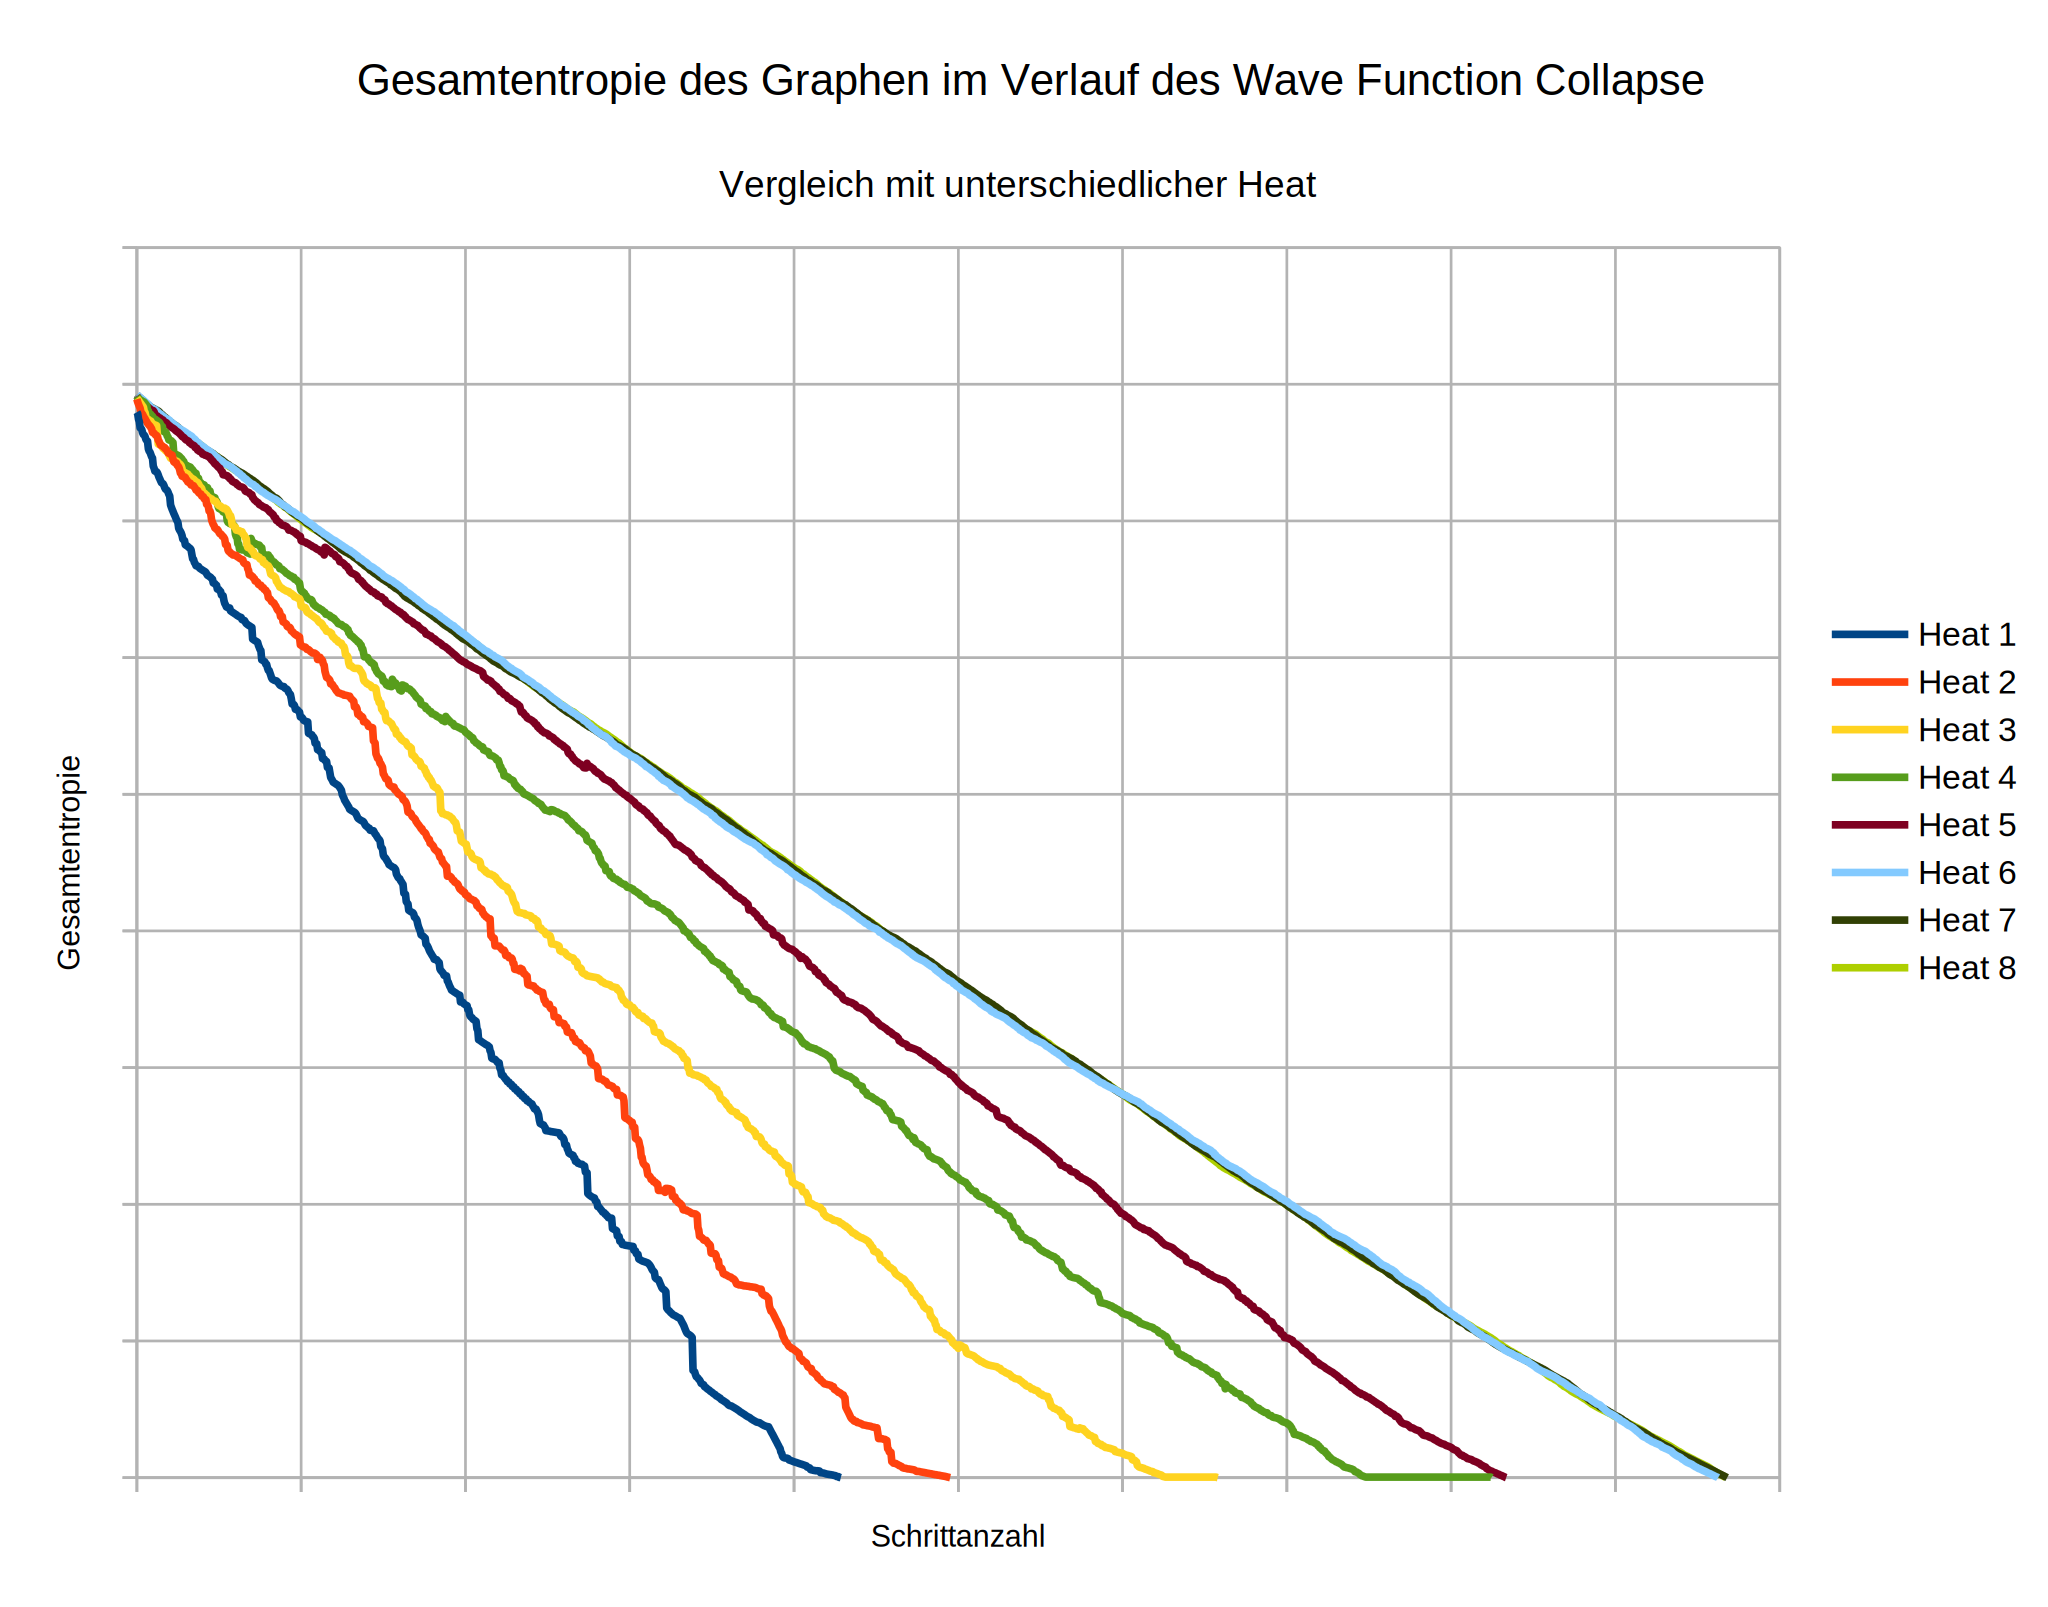
\includegraphics[width=\linewidth]{data/townscaper_grid/1.png} \caption{} \end{subfigure}
    \begin{subfigure}{0.18\textwidth} \includegraphics[width=\linewidth]{data/townscaper_grid/2.png} \caption{} \end{subfigure}
    \begin{subfigure}{0.18\textwidth} \includegraphics[width=\linewidth]{data/townscaper_grid/3.png} \caption{} \end{subfigure}
    \begin{subfigure}{0.18\textwidth} \includegraphics[width=\linewidth]{data/townscaper_grid/4.png} \caption{} \end{subfigure}
    \begin{subfigure}{0.18\textwidth} \includegraphics[width=\linewidth]{data/townscaper_grid/5.png} \caption{} \end{subfigure}
    
    \caption{
        Generierung eines Teils des Gitters für Townscaper \cite{stalberg_grid}. (a) Punkte werden generiert. (b) Triangulierung. (c) Kanten werden gelöscht, so dass Vierecke entstehen. (d) die Vierecke werden geviertelt. (e) Position der Knoten wird aufgelockert, so dass die Winkel zwischen Kanten gleichmäßiger sind.
    }
    \label{fig:townscaper_grid}
\end{figure}
        \begin{figure}[H]
    \centering
    \begin{minipage}{\linewidth}
        \rule{\linewidth}{0.4pt}
         
        \begin{enumerate}
        \item $M_0$ ist ein simples konsitentes Modell. $M = M_0$
        \subitem Wiederhole 2. bis 5. bis jeder Teil des Modells angepasst wurde
        \item Wähle eine Menge $B$ an Knotenpunkten zur Bearbeitung
        \item  $M' = M$ ohne die Knotenpunkte $B$ und deren bisherigen Bauteilen
        \item Arbeite alle Knotenpunkte von $B$ ab:
        \subitem Wähle einen Knotenpunkte aus und weise ihm ein konsistentes Bauteil zu
        \subitem Ist $M'$ nicht mehr konsistent, dann brich ab
        \subitem Füge diesen Knotenpunkt in $M'$ ein
        \item Wenn $M'$ noch konsistent ist, dann $M = M'$
        \end{enumerate}
        
        \rule{\linewidth}{0.4pt}
    \end{minipage}
    
    \caption{Model Synthesis Algorithmus nach Merrel \cite{merrel}}
    
    \label{fig:ms_merrel}
\end{figure}
        \begin{figure}[H]
    \centering
    \begin{subfigure}{0.18\textwidth} 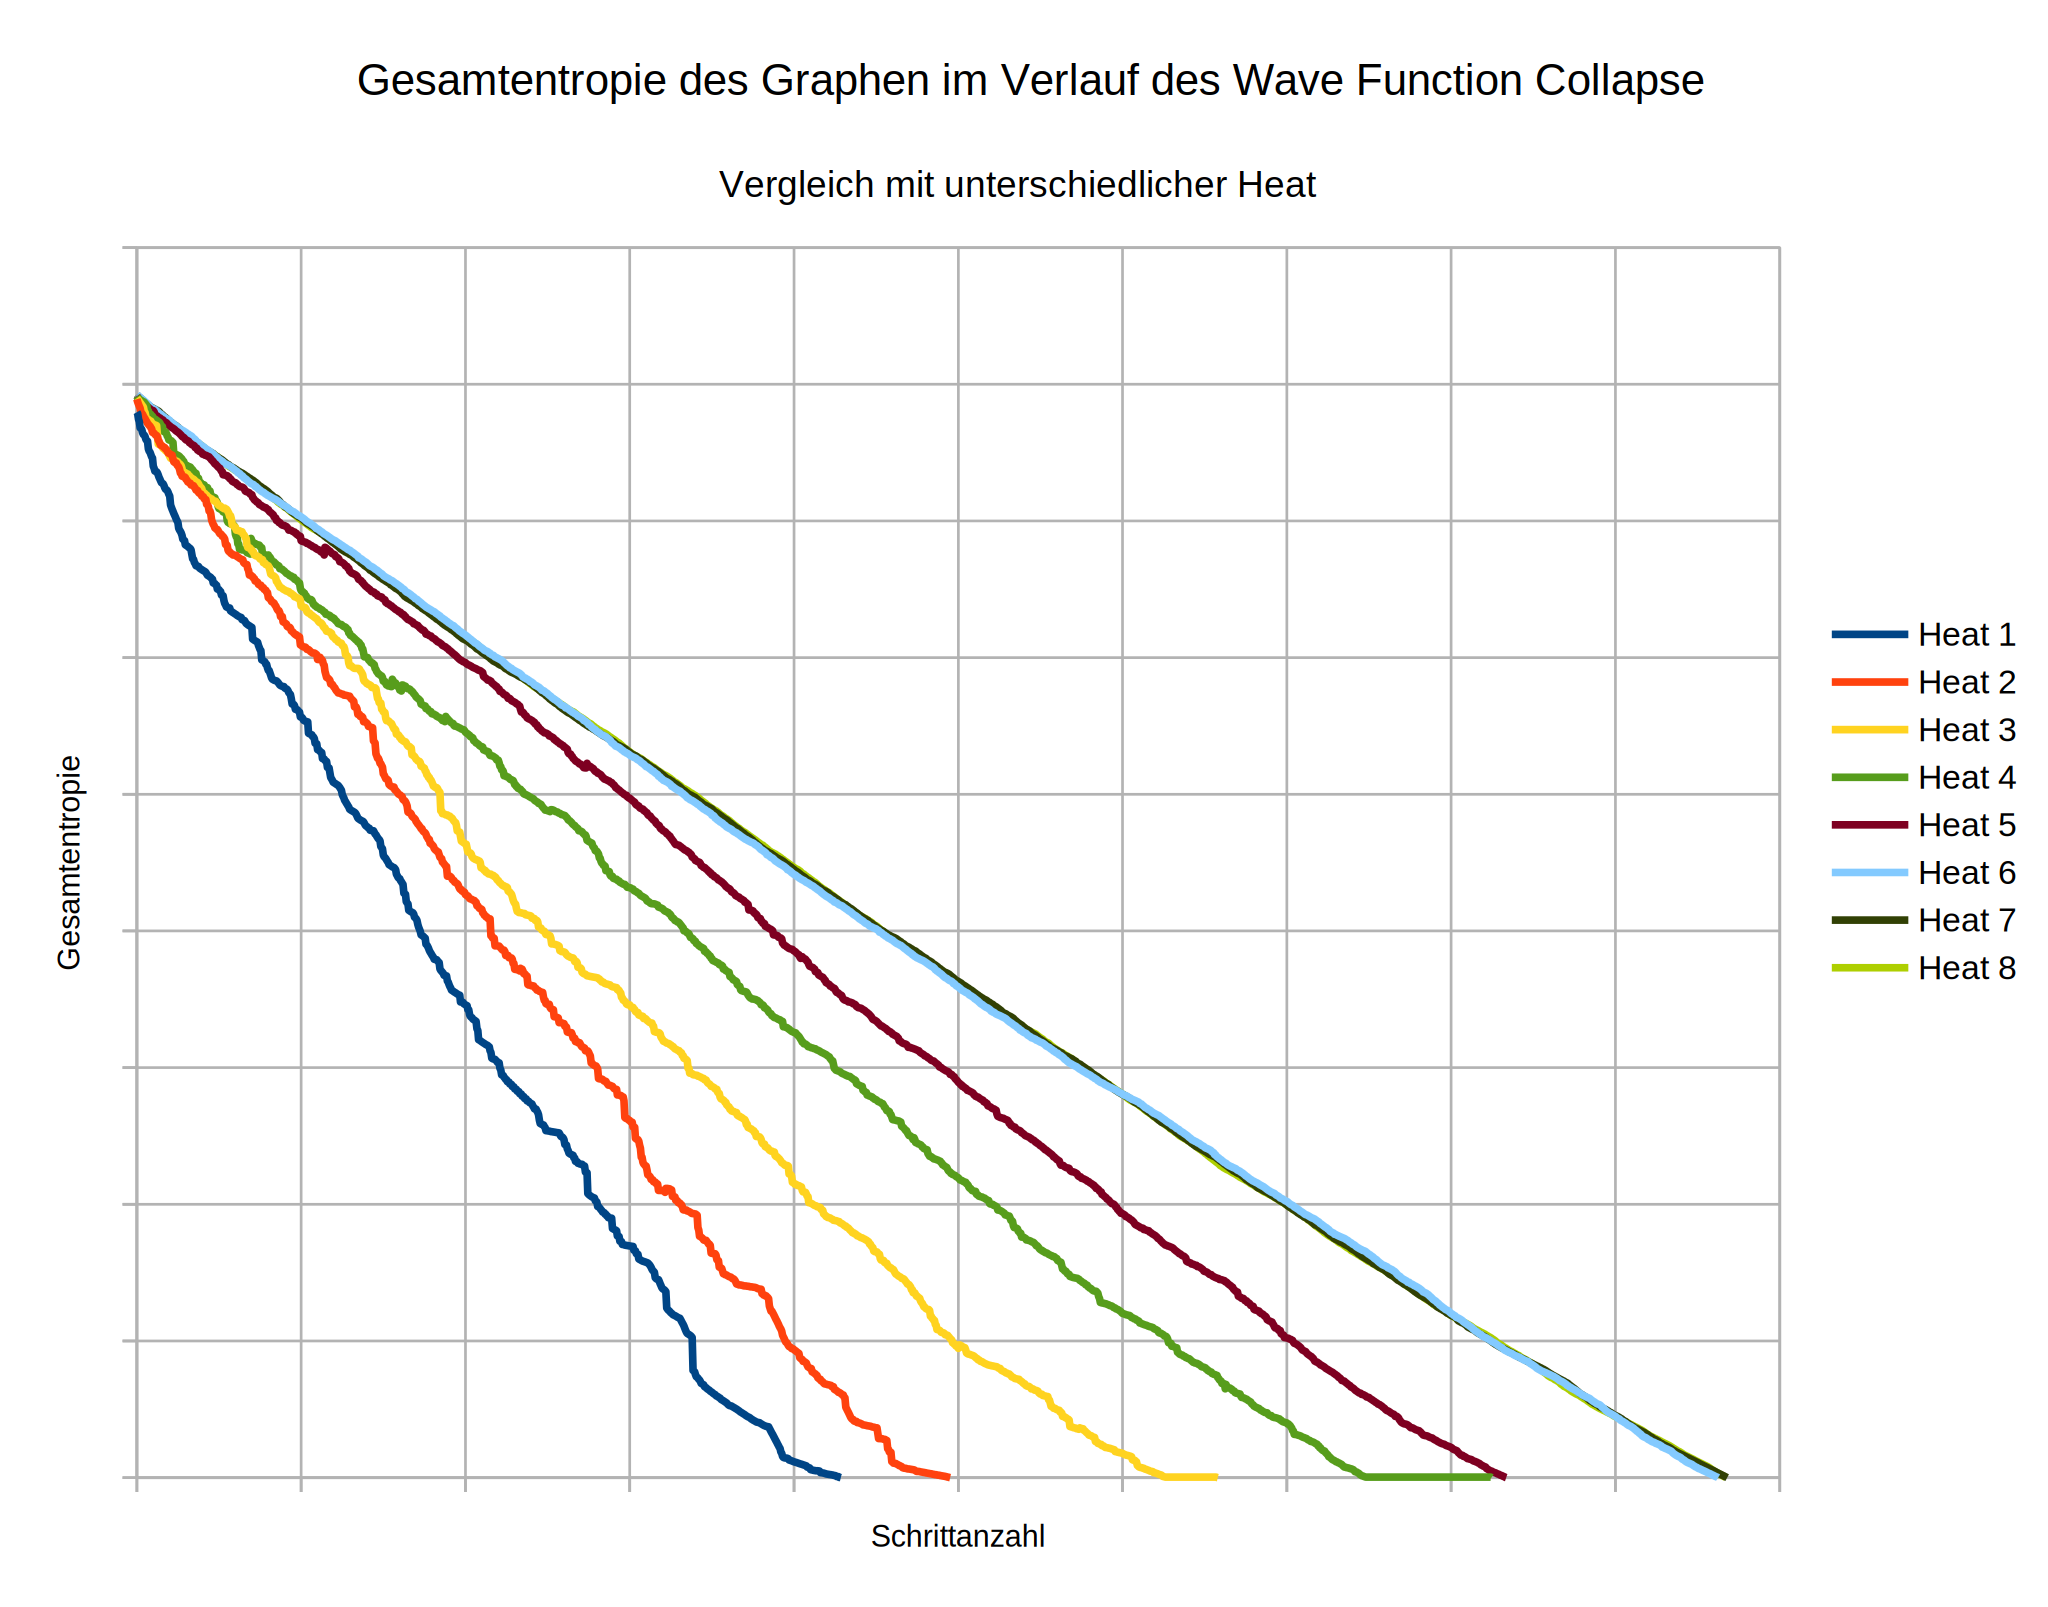
\includegraphics[width=\linewidth]{data/townscaper_grid/1.png} \caption{} \end{subfigure}
    \begin{subfigure}{0.18\textwidth} \includegraphics[width=\linewidth]{data/townscaper_grid/2.png} \caption{} \end{subfigure}
    \begin{subfigure}{0.18\textwidth} \includegraphics[width=\linewidth]{data/townscaper_grid/3.png} \caption{} \end{subfigure}
    \begin{subfigure}{0.18\textwidth} \includegraphics[width=\linewidth]{data/townscaper_grid/4.png} \caption{} \end{subfigure}
    \begin{subfigure}{0.18\textwidth} \includegraphics[width=\linewidth]{data/townscaper_grid/5.png} \caption{} \end{subfigure}
    
    \caption{
        Generierung eines Teils des Gitters für Townscaper \cite{stalberg_grid}. (a) Punkte werden generiert. (b) Triangulierung. (c) Kanten werden gelöscht, so dass Vierecke entstehen. (d) die Vierecke werden geviertelt. (e) Position der Knoten wird aufgelockert, so dass die Winkel zwischen Kanten gleichmäßiger sind.
    }
    \label{fig:townscaper_grid}
\end{figure}
        
        Die selbe Methodik kann auch für Beispielbilder benutzt werden, dies wird dann auch \textit{Texture Synthesis} genannt. In diesem Fall arbeitet der Algorithmus mit 2D Gittern und Bauteilen. Die Ausgabe des Algorithmus kann auch durch Soft-Constraints beschränkt werden (siehe Abbildung \ref{fig:ms_constrained}). Ebenso kann Symmetrie, Spiegelung und Drehung, in der Ausgabe erzwungen werden. Beide Ansätze wurden nicht weiter in dieser Arbeit betrachetet. Es wird empfohlen, dass der Algorithmus nicht das ganze Gitter auf einmal löst, damit Widersprüche nicht zu einem kompletten Neustart führen. Stattdessen sollen iterativ kleine Abschnitte für sich solange gelöst werden bis eine valide Ausgabe entsteht (siehe Abbildung \ref{fig:ms_algorithm}). In dieser Arbeit wurde darauf verzichtet.
        
        \begin{figure}[H]
    \centering
    \begin{subfigure}{0.18\textwidth} 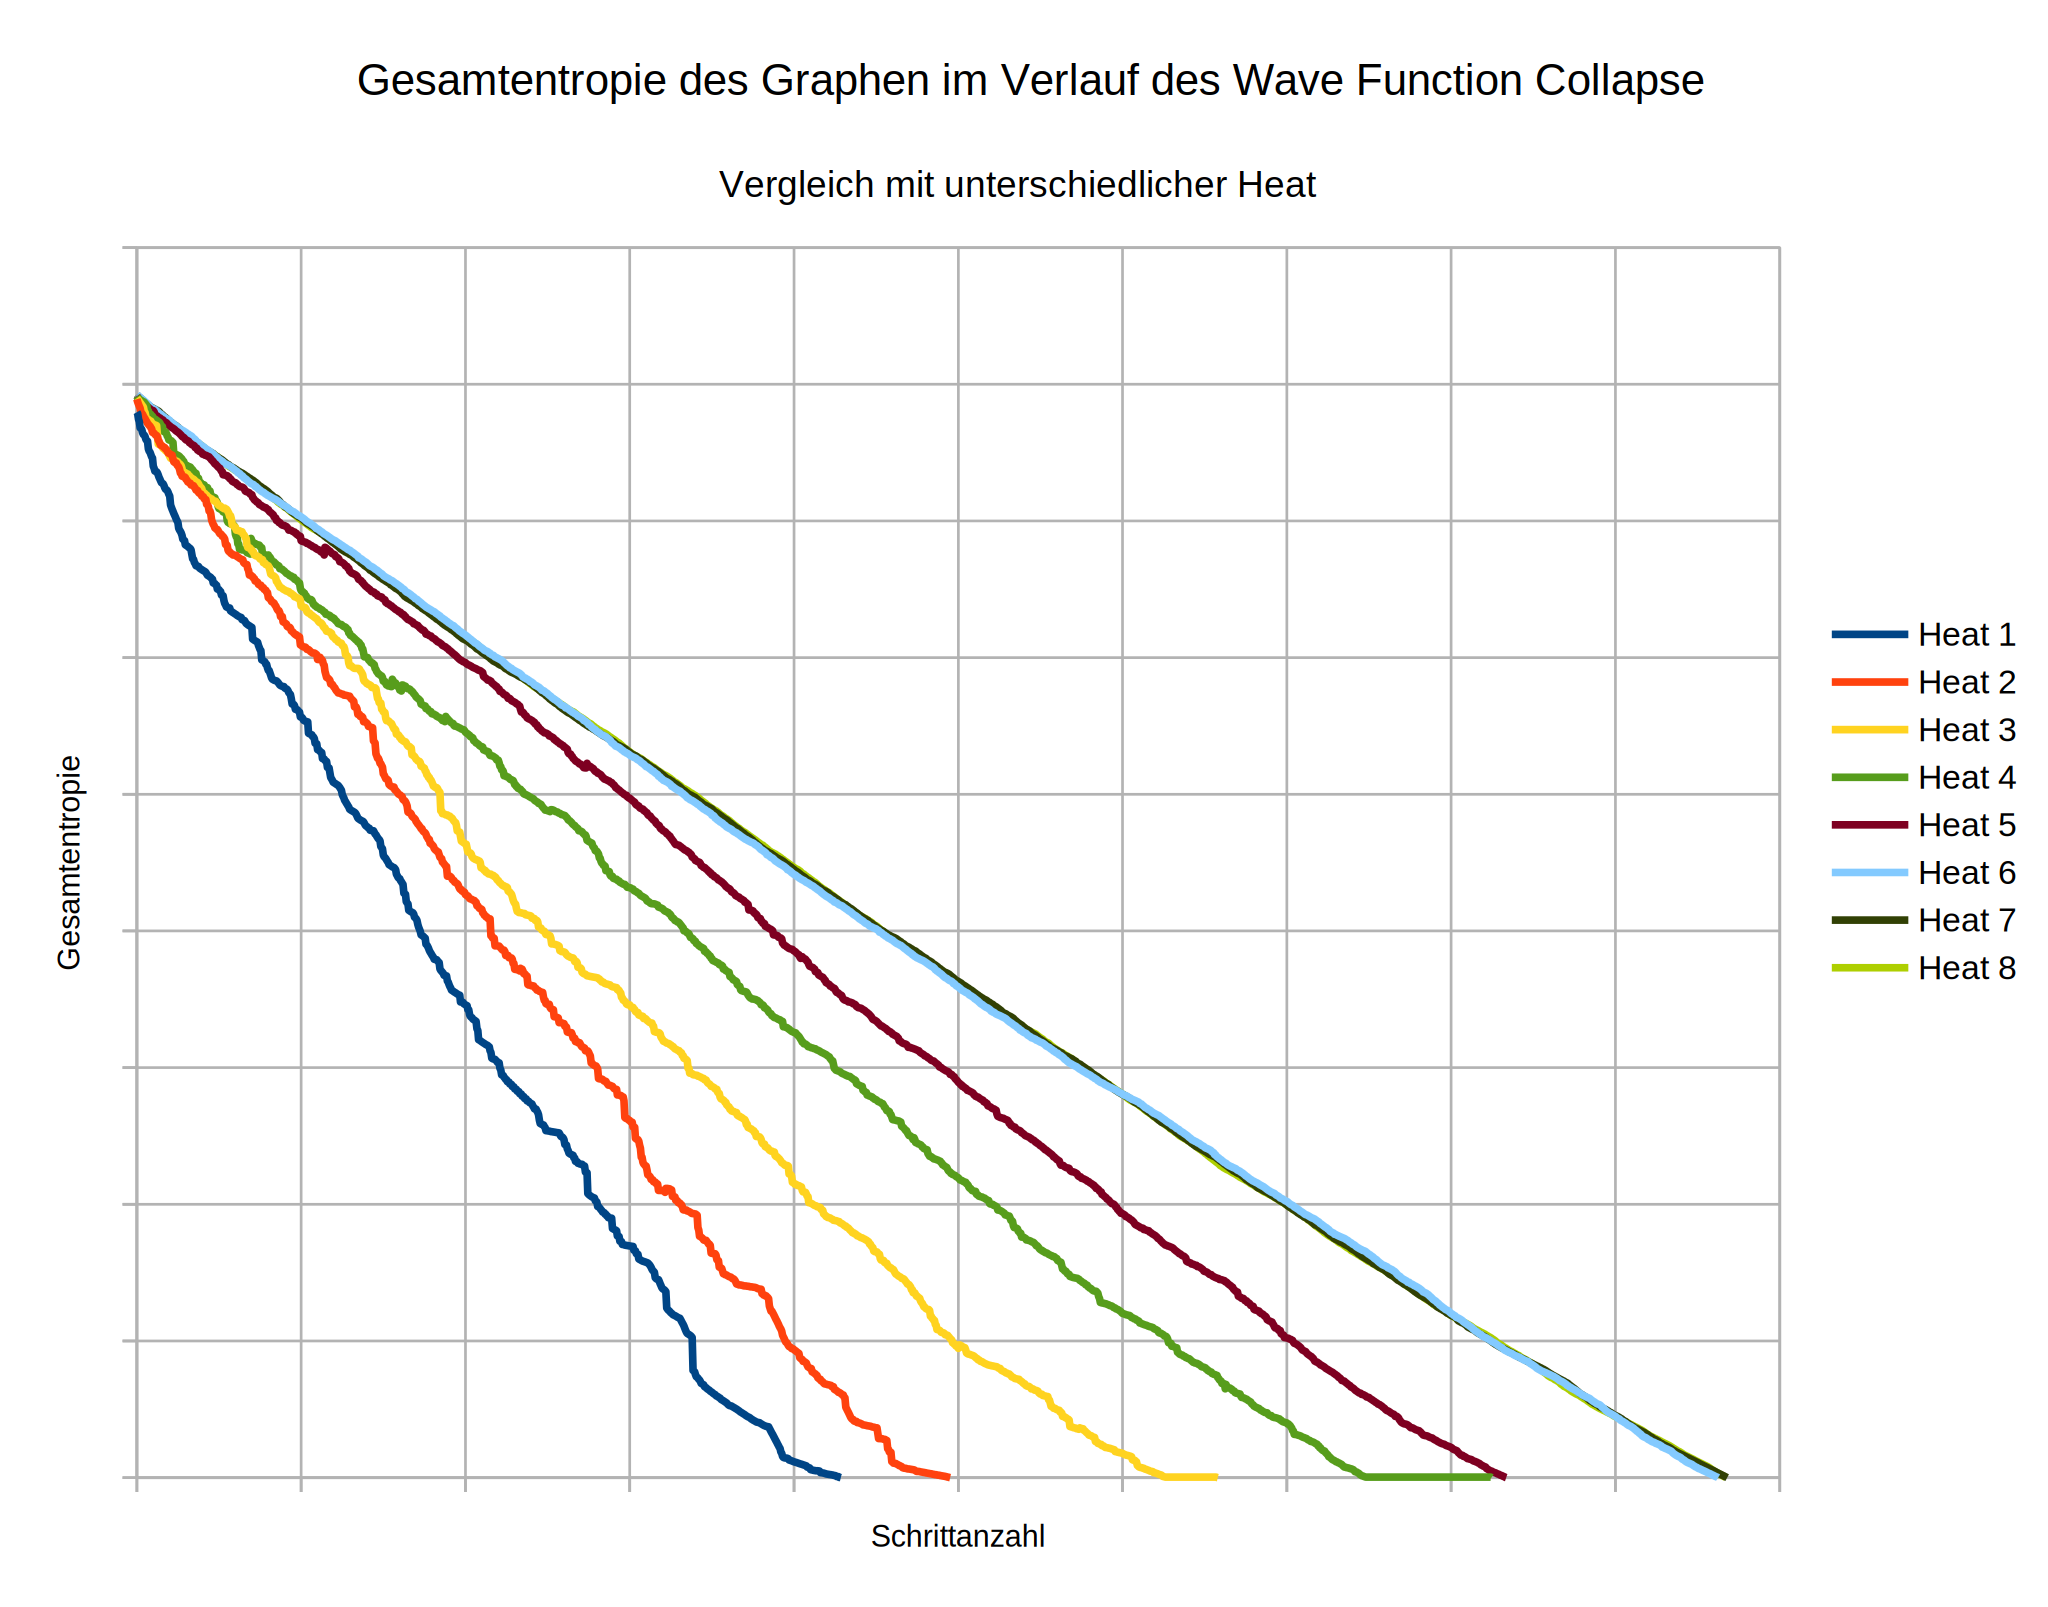
\includegraphics[width=\linewidth]{data/townscaper_grid/1.png} \caption{} \end{subfigure}
    \begin{subfigure}{0.18\textwidth} \includegraphics[width=\linewidth]{data/townscaper_grid/2.png} \caption{} \end{subfigure}
    \begin{subfigure}{0.18\textwidth} \includegraphics[width=\linewidth]{data/townscaper_grid/3.png} \caption{} \end{subfigure}
    \begin{subfigure}{0.18\textwidth} \includegraphics[width=\linewidth]{data/townscaper_grid/4.png} \caption{} \end{subfigure}
    \begin{subfigure}{0.18\textwidth} \includegraphics[width=\linewidth]{data/townscaper_grid/5.png} \caption{} \end{subfigure}
    
    \caption{
        Generierung eines Teils des Gitters für Townscaper \cite{stalberg_grid}. (a) Punkte werden generiert. (b) Triangulierung. (c) Kanten werden gelöscht, so dass Vierecke entstehen. (d) die Vierecke werden geviertelt. (e) Position der Knoten wird aufgelockert, so dass die Winkel zwischen Kanten gleichmäßiger sind.
    }
    \label{fig:townscaper_grid}
\end{figure}
    
    
    \section{Wave Function Collapse}
        \textit{Wave Function Collapse} ist eine Weiterentwicklung des Model Sythesis Algorithmus \cite{gumin}. Der Name ist eine Anspielung auf die Quantenphysik. So könnte man Quantenpartikel in Superposition mit den Zellen des Gitters vergleichen. Die Zellen haben auch mehrere mögliche finale Zustände bis sie observiert werden und in einen festen Zustand collapsen. Mathematisch besteht aber keine Beziehung. Auch werden andere Begriffe wie z.B. Knoten zu Zelle umbenannt und das Gitter als Wave bezeichnet. Die Kernidee der Generierung mittels einem Beispiel bleibt und wird um drei Aspekte erweitert:
        
        \begin{enumerate}
        \item Bauteile können automatisch aus einem Beispiel extrahiert werden.
        \item Im Algorithmus werden die Zellen beginnend mit der niedrigsten Entropie abgearbeitet. 
        \item Spiegelungen und Reflexionen von Bauteilen werden automatisch erzeugt und verwendet.
        \end{enumerate}
        
        Der Algorithmus ist in Abbildung \ref{fig:wfc_gumin} dargestellt. Abbildung \ref{fig:wfc_overview} zeigt ein paar Beispiele und daraus generierte Bilder.
        
        \begin{figure}[ht]
    \centering
    \begin{minipage}{\linewidth}
        \rule{\linewidth}{0.4pt}
        
        \begin{enumerate}
        \item Read the input bitmap and count NxN patterns.
        \subitem (optional) Augment pattern data with rotations and reflections.
        \item Create an array with the dimensions of the output (called ''wave'' in the source). Each element of this array represents a state of an NxN region in the output. A state of an NxN region is a superposition of NxN patterns of the input with boolean coefficients (so a state of a pixel in the output is a superposition of input colors with real coefficients). False coefficient means that the corresponding pattern is forbidden, true coefficient means that the corresponding pattern is not yet forbidden.
        \item Initialize the wave in the completely unobserved state, i.e. with all the boolean coefficients being true.
        \item Repeat the following steps: \begin{enumerate}
            \item Observation: \begin{enumerate}
                \item Find a wave element with the minimal nonzero entropy. If there is no such elements (if all elements have zero or undefined entropy) then break the cycle (4) and go to step (5).
                \item Collapse this element into a definite state according to its coefficients and the distribution of NxN patterns in the input.
            \end{enumerate}
            \item Propagation: propagate information gained on the previous observation step.
        \end{enumerate}
        \item By now all the wave elements are either in a completely observed state (all the coefficients except one being zero) or in the contradictory state (all the coefficients being zero). In the first case return the output. In the second case finish the work without returning anything.
        \end{enumerate}
        
        \rule{\linewidth}{0.4pt}
    \end{minipage}
    
    \caption{Wave Function Collapse Algorithmus nach Gumin \cite{gumin}}
    
    \label{fig:wfc_gumin}
\end{figure}
        \begin{figure}[H]
    \centering
    \begin{subfigure}{0.18\textwidth} 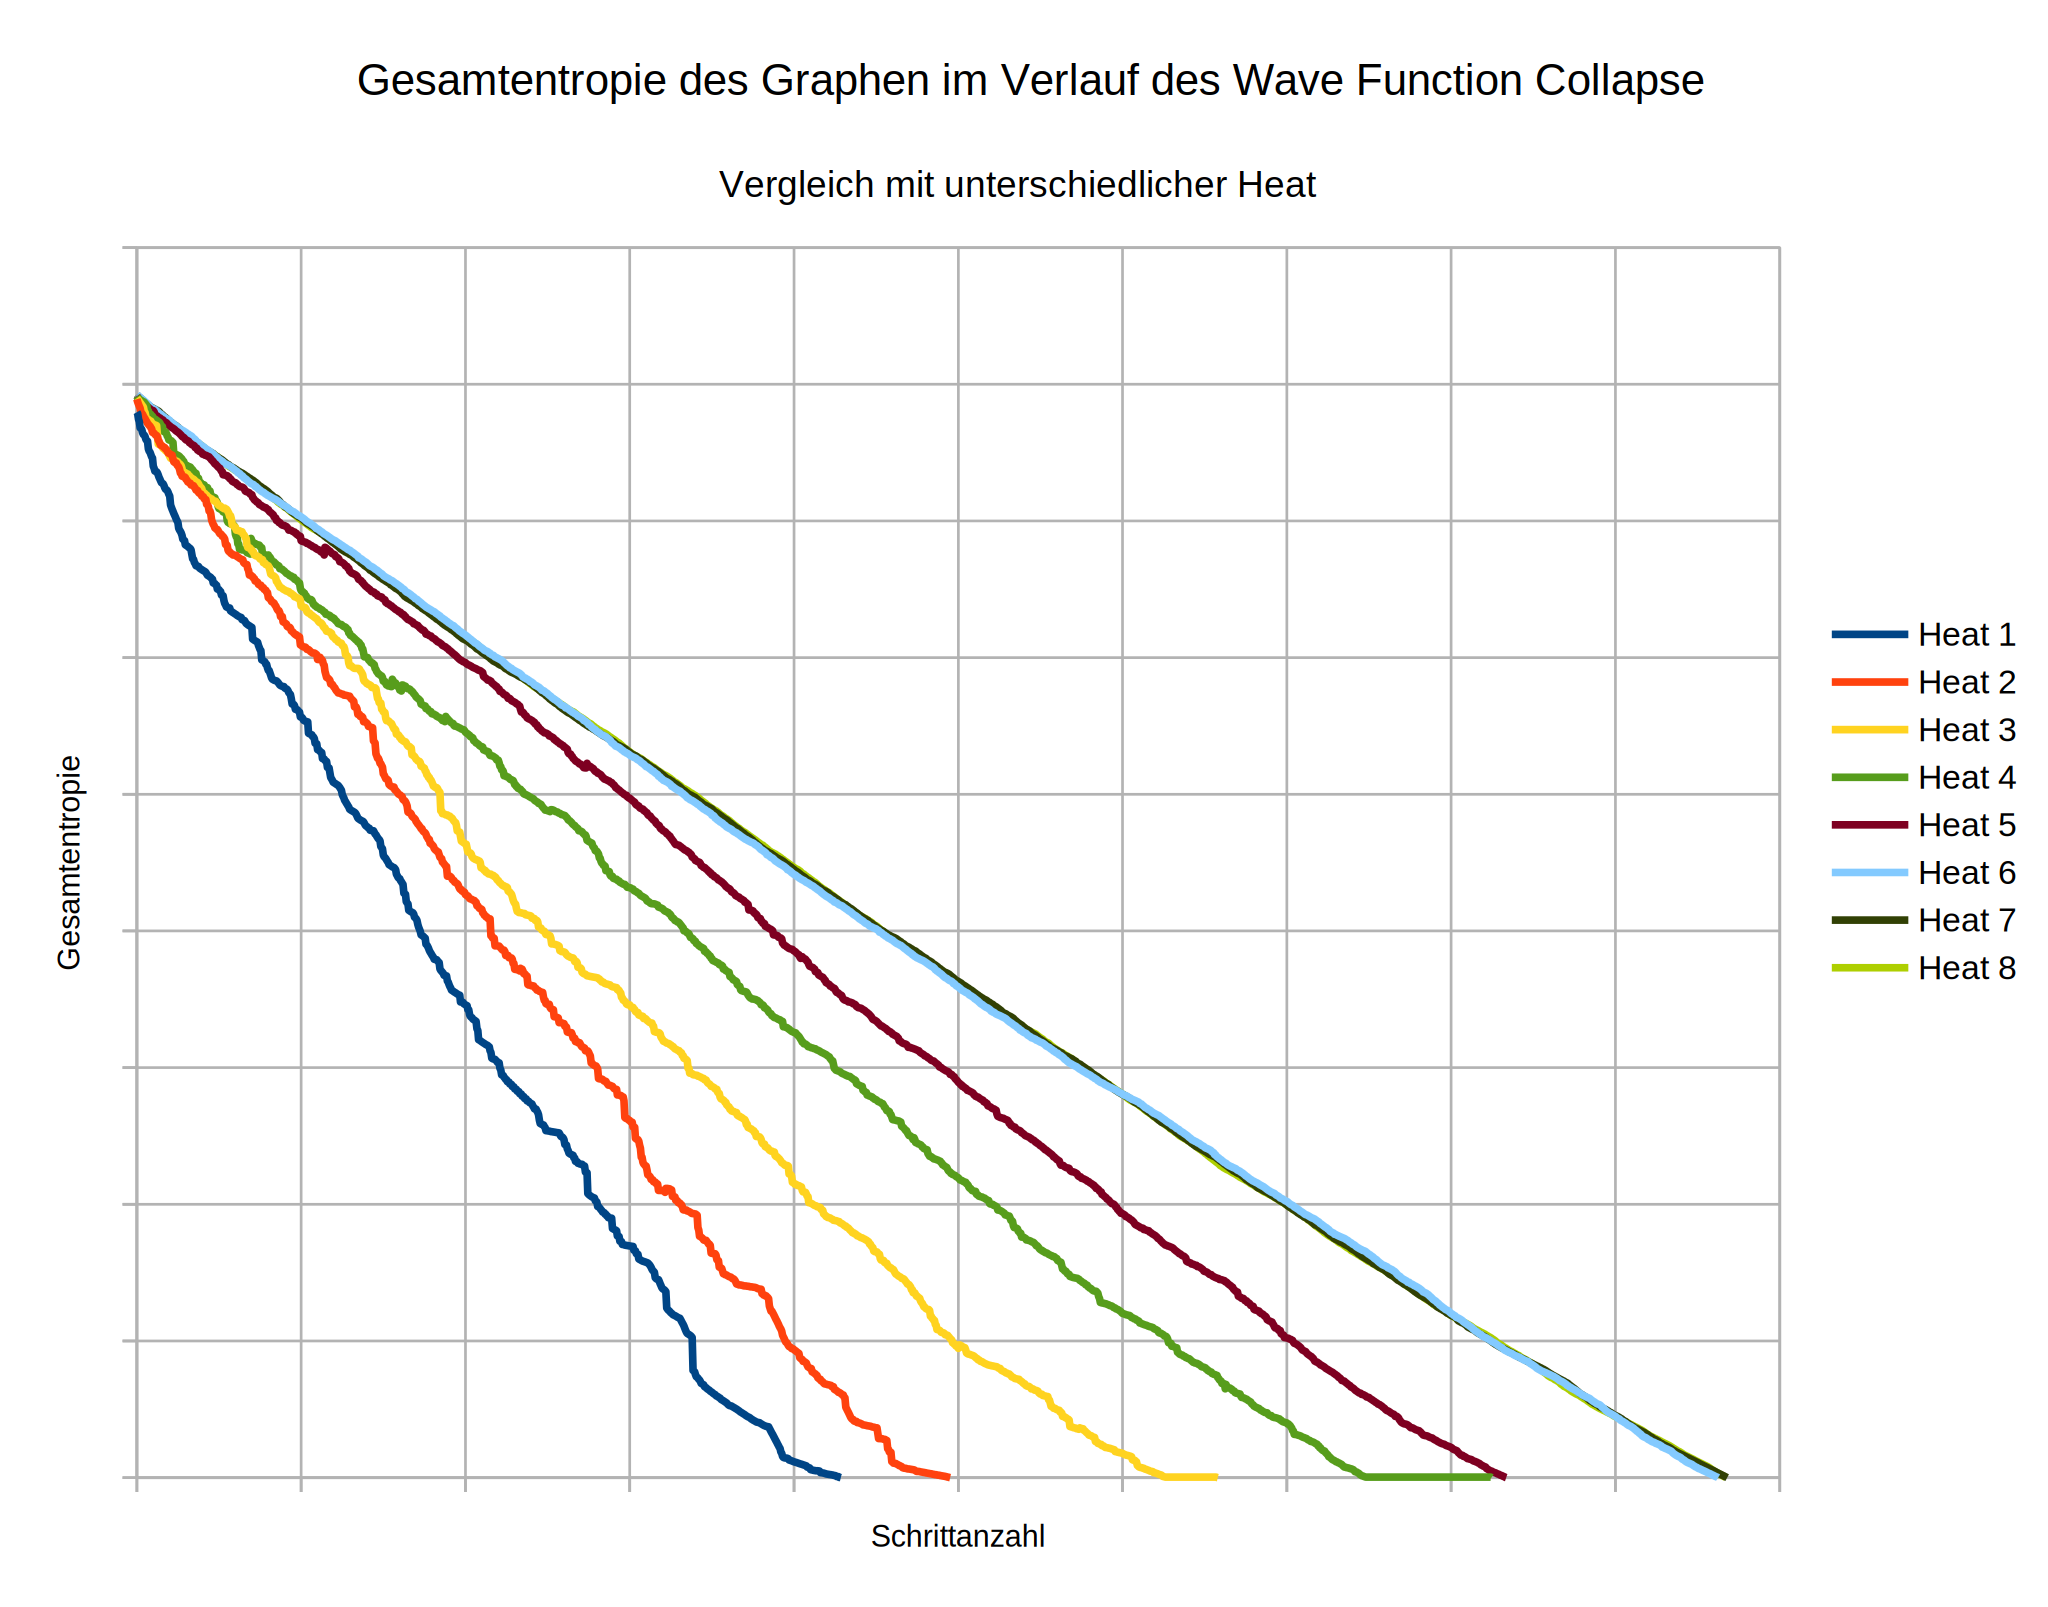
\includegraphics[width=\linewidth]{data/townscaper_grid/1.png} \caption{} \end{subfigure}
    \begin{subfigure}{0.18\textwidth} \includegraphics[width=\linewidth]{data/townscaper_grid/2.png} \caption{} \end{subfigure}
    \begin{subfigure}{0.18\textwidth} \includegraphics[width=\linewidth]{data/townscaper_grid/3.png} \caption{} \end{subfigure}
    \begin{subfigure}{0.18\textwidth} \includegraphics[width=\linewidth]{data/townscaper_grid/4.png} \caption{} \end{subfigure}
    \begin{subfigure}{0.18\textwidth} \includegraphics[width=\linewidth]{data/townscaper_grid/5.png} \caption{} \end{subfigure}
    
    \caption{
        Generierung eines Teils des Gitters für Townscaper \cite{stalberg_grid}. (a) Punkte werden generiert. (b) Triangulierung. (c) Kanten werden gelöscht, so dass Vierecke entstehen. (d) die Vierecke werden geviertelt. (e) Position der Knoten wird aufgelockert, so dass die Winkel zwischen Kanten gleichmäßiger sind.
    }
    \label{fig:townscaper_grid}
\end{figure}
        
        
        \subsection{Entropie}
            Bei Model Synthesis werden Zellen einfach nach ihrer Reihenfolge im Gitter abgearbeitet. Der Vorteil ist, dass keine Suche der nächsten Zelle nötig ist, aber es hat zum Nachteil, dass die Ausgabe sichtbare Artefakte enthällt (siehe Abbildung \ref{fig:directional_bias}). Man kann erkennen, ob zuerst die Reihen oder erst die Spalten abgearbeitet wurden. Wäre bekannt welche Zelle den meisten Fortschritt zur Lösung und die geringste Chance auf einen Widerspruch birgt, könnte stets diese Zelle zuerst betrachtet werden. Doch Merrel zeigt im Anhang seines Papers \cite{merrel}, dass die Entscheidung, ob eine Ausgabe vervollständigt werden kann, ein NP-vollständiges Problem ist. 
            
            \begin{figure}[H]
    \centering
    \begin{subfigure}{0.18\textwidth} 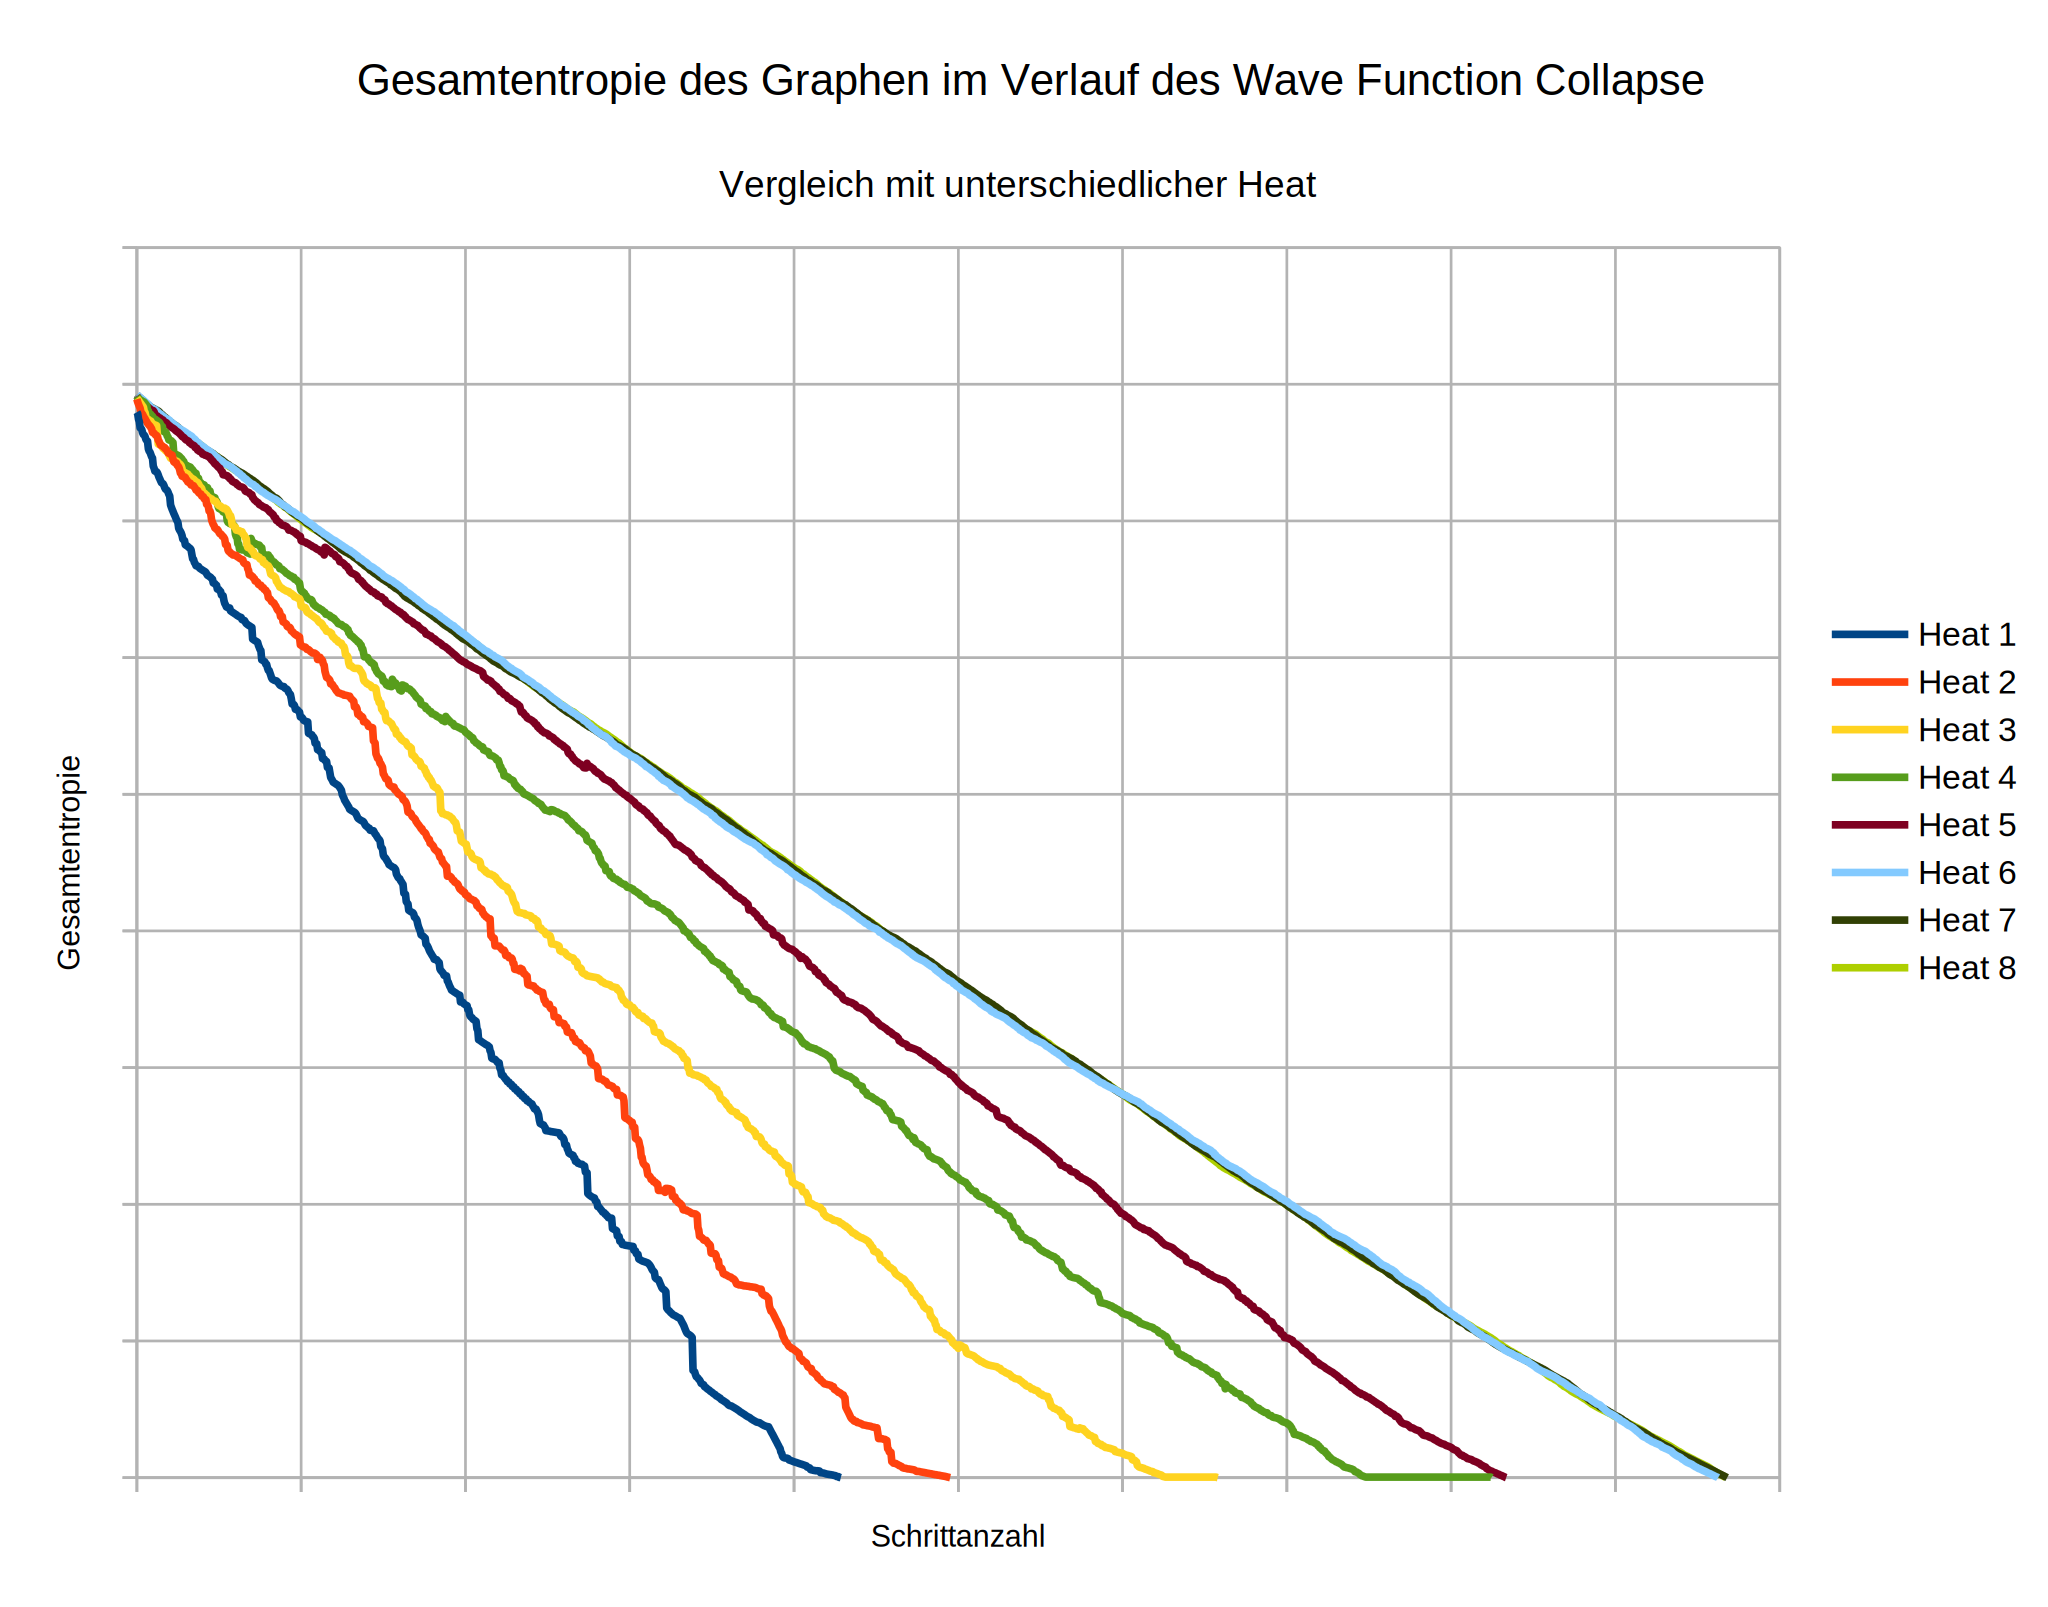
\includegraphics[width=\linewidth]{data/townscaper_grid/1.png} \caption{} \end{subfigure}
    \begin{subfigure}{0.18\textwidth} \includegraphics[width=\linewidth]{data/townscaper_grid/2.png} \caption{} \end{subfigure}
    \begin{subfigure}{0.18\textwidth} \includegraphics[width=\linewidth]{data/townscaper_grid/3.png} \caption{} \end{subfigure}
    \begin{subfigure}{0.18\textwidth} \includegraphics[width=\linewidth]{data/townscaper_grid/4.png} \caption{} \end{subfigure}
    \begin{subfigure}{0.18\textwidth} \includegraphics[width=\linewidth]{data/townscaper_grid/5.png} \caption{} \end{subfigure}
    
    \caption{
        Generierung eines Teils des Gitters für Townscaper \cite{stalberg_grid}. (a) Punkte werden generiert. (b) Triangulierung. (c) Kanten werden gelöscht, so dass Vierecke entstehen. (d) die Vierecke werden geviertelt. (e) Position der Knoten wird aufgelockert, so dass die Winkel zwischen Kanten gleichmäßiger sind.
    }
    \label{fig:townscaper_grid}
\end{figure}
            
            Einfacher ist es eine Heuristik zu definieren. Hierfür wird die Shannon-Entropie \cite{shannon} als Maß eingeführt. Sie beschreibt das Maß an Ungewissheit in einem System, hier die Ungewissheit über den finalen Zustand einer Zelle. Ist eine Zelle observiert, hat sie nur noch einen Zustand und die Entropie ist 0, während eine Zelle mit vielen Möglichkeiten eine hohe Entropie hat. Die Entropie gibt auch Information darüber wie sehr eine Zelle durch ihre Umgebung beschränkt wird, weil Zellen mit vielen Beschränkungen nur noch wenige mögliche Zustände haben.             
            %     % \caption{
%     %     Formel für die Shannon-Entropie. 
%     %     $\mathcal{X}$ ist die Menge der Möglichen Zustände einer Zelle.
%     %     $p(x)$ ist die Wahrscheinlichkeit das $x$ gewählt wird.
%     % }

\begin{equation}
    \label{eq:entropy}
    \mathrm{entropy}(\mathcal{X}) = -\sum_{x \in \mathcal{X}} p(x),\log p(x)
\end{equation}
        
        
        \subsection{Symmetrie}
            Ziel des Model Synthesis Algorithmus ist es, eine große Anzahl lokal ähnlicher Ausgaben zu generieren \cite{merrel}. Ähnlichkeit wird erreicht, wenn jede kleine Region der Ausgabe zu Regionen des Beispiels passt \ref{fig:wfc_resemblance}. Die wahrgenommene Ähnlichkeit wird verbessert, wenn das Verhältnis der Häufigkeiten von Regionen der Verteilung im Beispiel gleicht. Im Wave Function Collapse wird dieses Kriterium erweitert. Die Regionen können nun auch Drehungen und Spiegelungen der Regionen im Beispiel sein \cite{gumin}.
            
            \begin{figure}[H]
    \centering
    \begin{subfigure}{0.18\textwidth} 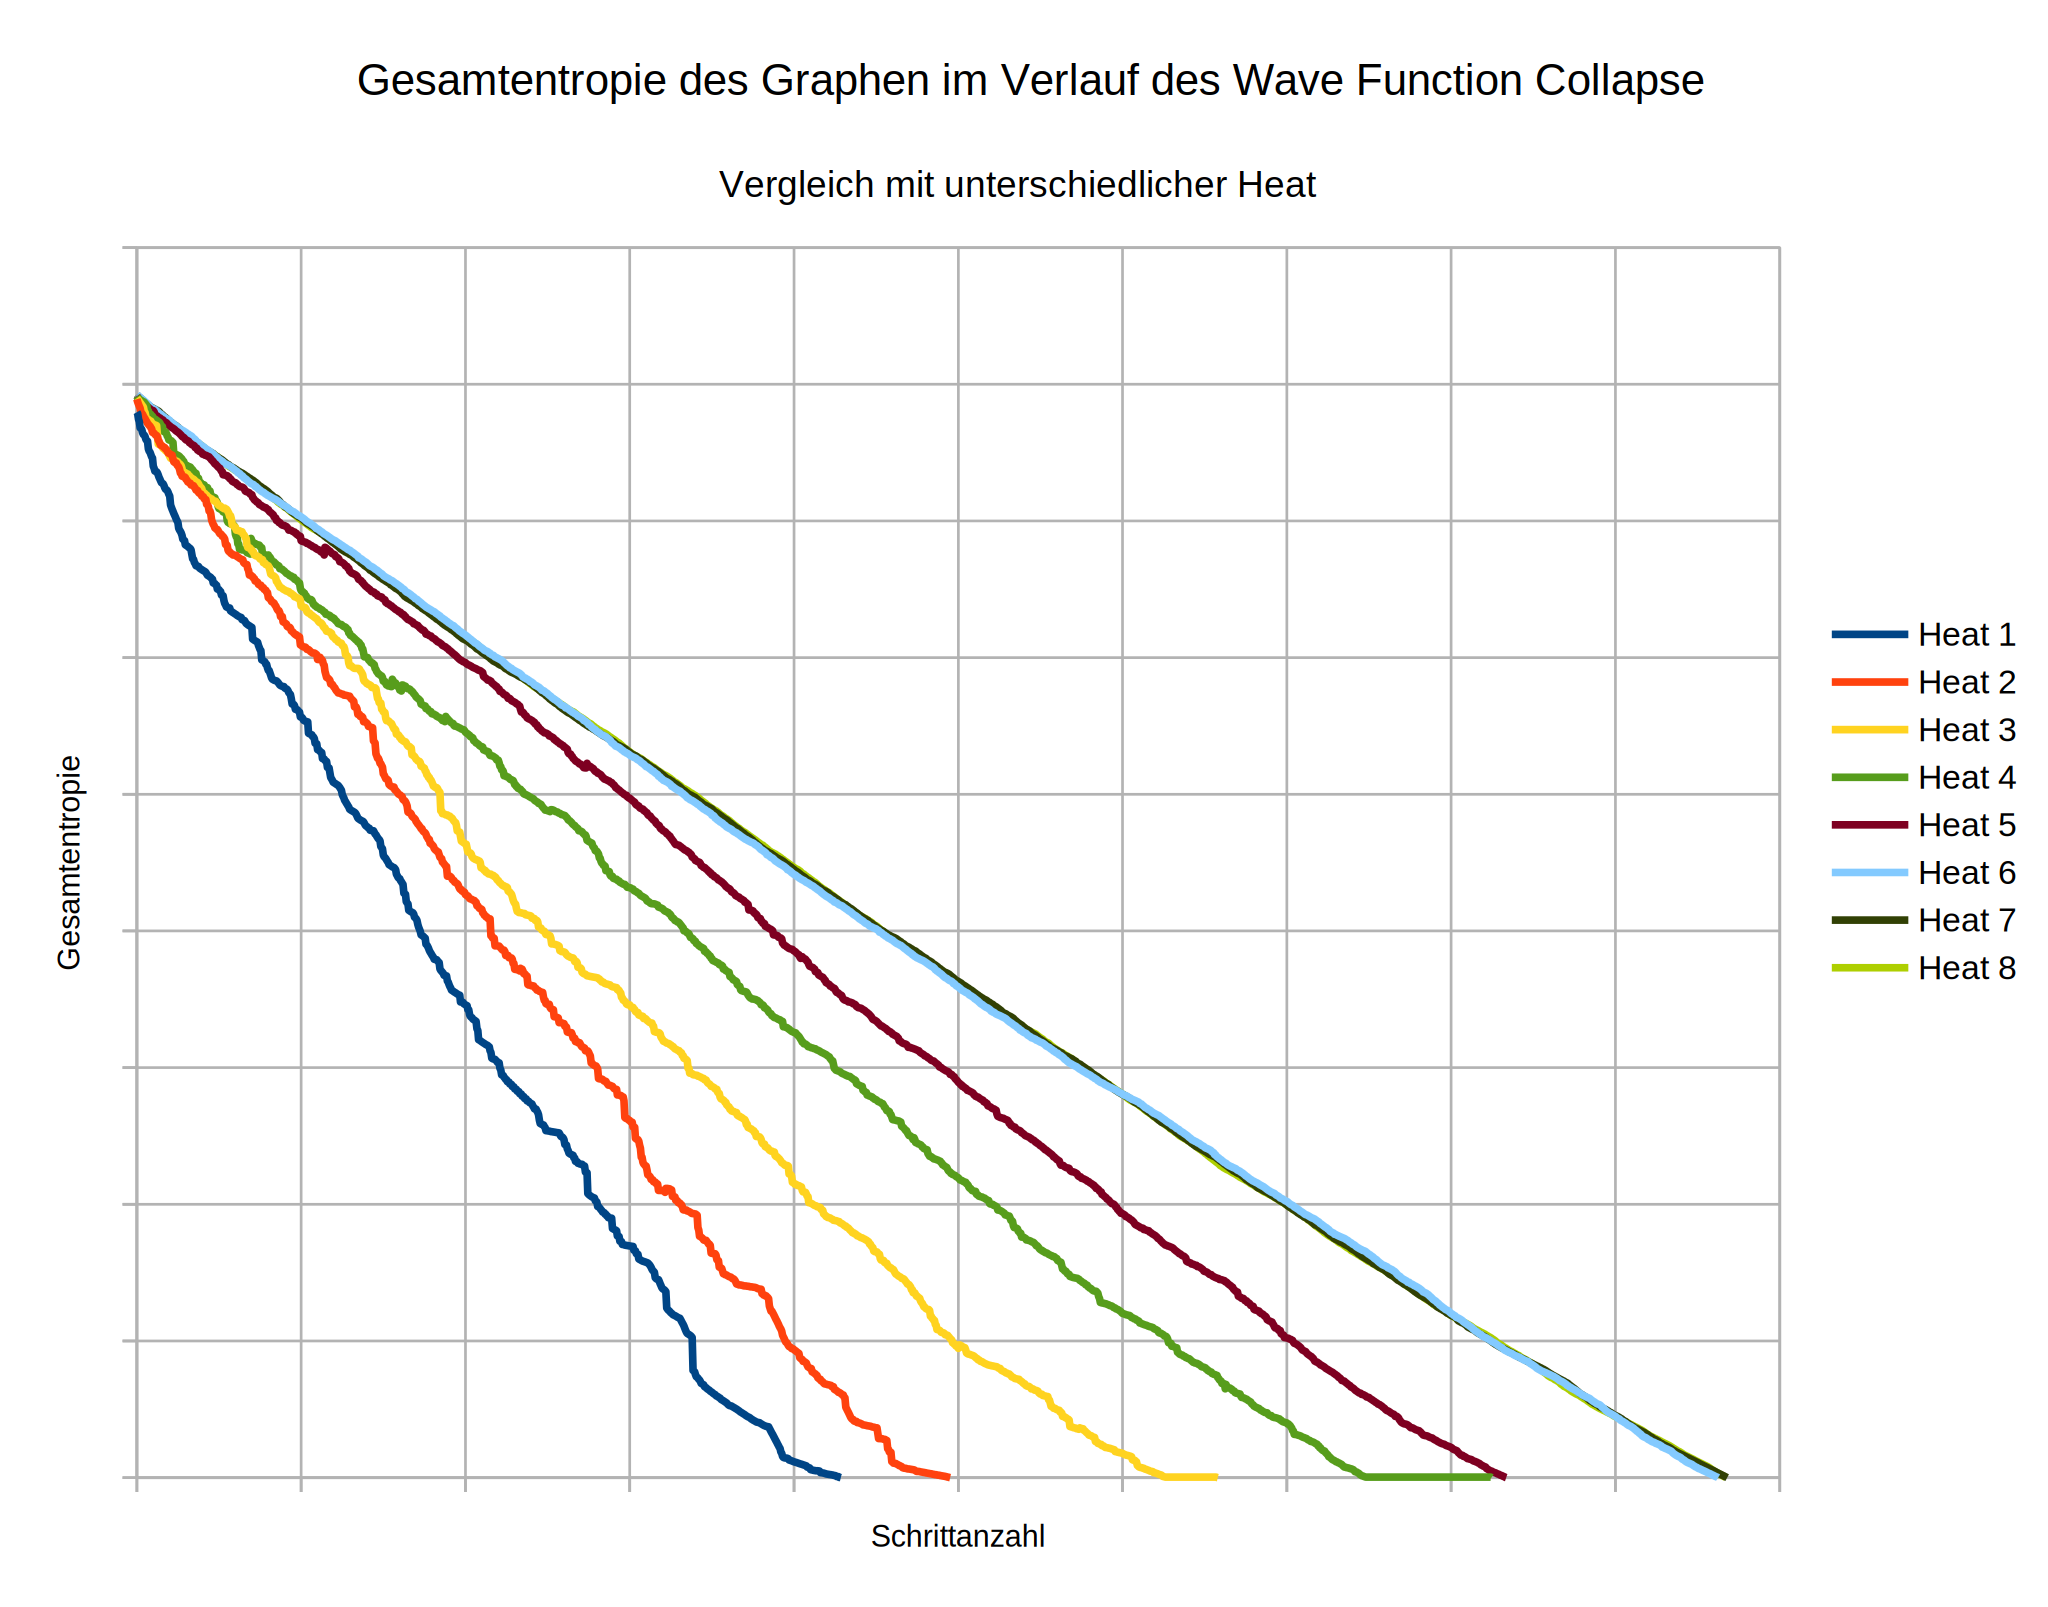
\includegraphics[width=\linewidth]{data/townscaper_grid/1.png} \caption{} \end{subfigure}
    \begin{subfigure}{0.18\textwidth} \includegraphics[width=\linewidth]{data/townscaper_grid/2.png} \caption{} \end{subfigure}
    \begin{subfigure}{0.18\textwidth} \includegraphics[width=\linewidth]{data/townscaper_grid/3.png} \caption{} \end{subfigure}
    \begin{subfigure}{0.18\textwidth} \includegraphics[width=\linewidth]{data/townscaper_grid/4.png} \caption{} \end{subfigure}
    \begin{subfigure}{0.18\textwidth} \includegraphics[width=\linewidth]{data/townscaper_grid/5.png} \caption{} \end{subfigure}
    
    \caption{
        Generierung eines Teils des Gitters für Townscaper \cite{stalberg_grid}. (a) Punkte werden generiert. (b) Triangulierung. (c) Kanten werden gelöscht, so dass Vierecke entstehen. (d) die Vierecke werden geviertelt. (e) Position der Knoten wird aufgelockert, so dass die Winkel zwischen Kanten gleichmäßiger sind.
    }
    \label{fig:townscaper_grid}
\end{figure}
            
            Desweiteren wird auch eine Annotation für manuell erstellten Bauteile definiert, mit der ein Nutzer einem Bauteil eine Symmetriegruppe zuweisen kann \cite{gumin}. Eine Symmetriegruppe gibt an, wie man ein Bauteil drehen und spiegeln kann. Beim Einlesen generiert der Algorithmus basiert auf dieser Symmetriegruppe weitere, entsprechend gedreht oder gespiegelte, Bauteil die im weiteren Prozess verwendet werden. Da sich diese Arbeit nicht mit Beispielen aus Bauteilen befässt sondern primär diese automatisch extrahiert, bleibt dieser Aspekt ungenutzt.
        
        
        \subsection{Extraktion}
            Zuvor musste der Nutzer das gewünschte Beispielmodell oder Beispielbild manuell in einzelne gleichgroße Bauteile zerlegen, aus denen der Algorithmus dann neue Modelle und Bilder generiert. Wave Function Collapse nutzt einen Algorithmus \ref{fig:wfc_extraction} zur Generierung dieser Bauteile \cite{gumin}. Die größe der Bauteile ist dabei freiwählbar, aber sie sollte so gewählt sein, das sie zum genutzen Beispiel passt, damit die im Beispiel existierenden Muster erhalten bleiben.  Sind die Bauteile zu klein gewählt, gehen Strukturen des Beispiels verloren. Während zu große Bauteile auch unerwünschte Strukturen im Beispiel enthalten, was im extremen Fall dazu führt, dass nur noch exakte Kopien des Beispiels ohne Variation in der Ausgabe vorkommen. Für Bilder wird in dieser Arbeit stets die Moore-Nachbarschaft jedes Pixels, also die direkt angrenzenden Pixel sowie die entlang der Diagonalen, als Bauteil verwendet. Dies wird auch als das Umfeld des Pixels beschrieben.
            
            \begin{algorithm}
    \caption{Regelextraktion}
    \label{alg:wfc_extraction}
    
    \begin{enumerate}
    \item Für jeden Pixel des Beispielbilds:
        \begin{enumerate}
        \item Überschreitet das Umfeld des Pixels den Rand des Bild?
        \subitem Ist Wrapping erlaubt?
        \subsubitem Dann: Nimm die Pixel vom gegenüberliegenden Rand
        \subsubitem Sonst: Überspringe diesen Pixel
        \item Lese das Umfeld aus
        \item Gibt es bereits einen Zustand mit diesem Umfeld?
        \subitem Dann: Erhöhe dessen Frequenz um eins
        \subitem Sonst: Erstelle einen neuen Zustand mit diesem Umfeld
        \end{enumerate}
    
    \item Für jedes Paar Zustände und jede Himmelsrichtung:
        \begin{enumerate}
        \item Prüfe ob die Zustände in dieser Richtung überlappen
        \item Speichere diese Regel in der Lookuptabelle ab
        \end{enumerate}
    \end{enumerate}
        
\end{algorithm}
            
            In Abbildung \ref{fig:extract_wrapping} ist der Ablauf dargestellt. Aus dem Beispiel werden die Umfelder ausgelesen. In der Abbildung wird vertikales Wrapping \at{@translation} genutzt, ist das vom Nutzer nicht erwünscht so würden Umfelder die den Rand des Beispiels überschreiten einfach verworfen und nicht weiter verwendet. Die Zustände ergeben sich aus den einzigartigen Umfelder. Die Frequenz eines Umfelds gibt an wie oft es im Beispiel vorkommt. Sind mehrere Umfelder gleich, so hat der entsprechende Zustand einen höhere Frequenz. Aus der Gesamtanzahl an Zuständen und deren Frequenzen lässt sich die Wahrscheinlichkeit jedes Zustands berechen. Im Algorithmus wird dies beachtet, damit auch die globale Verteilung von Umfeldern in der Ausgabe der Verteilung im Beispiel ähnelt. Danach wird geprüft welche der gefundenen Umfelder überlappen. Es werden die Himmelrichtungen N, S, W und O geprüft und für später in einer Lookuptabelle gespeichert.
            
            \begin{figure}[H]
    \centering
    \begin{subfigure}{0.18\textwidth} 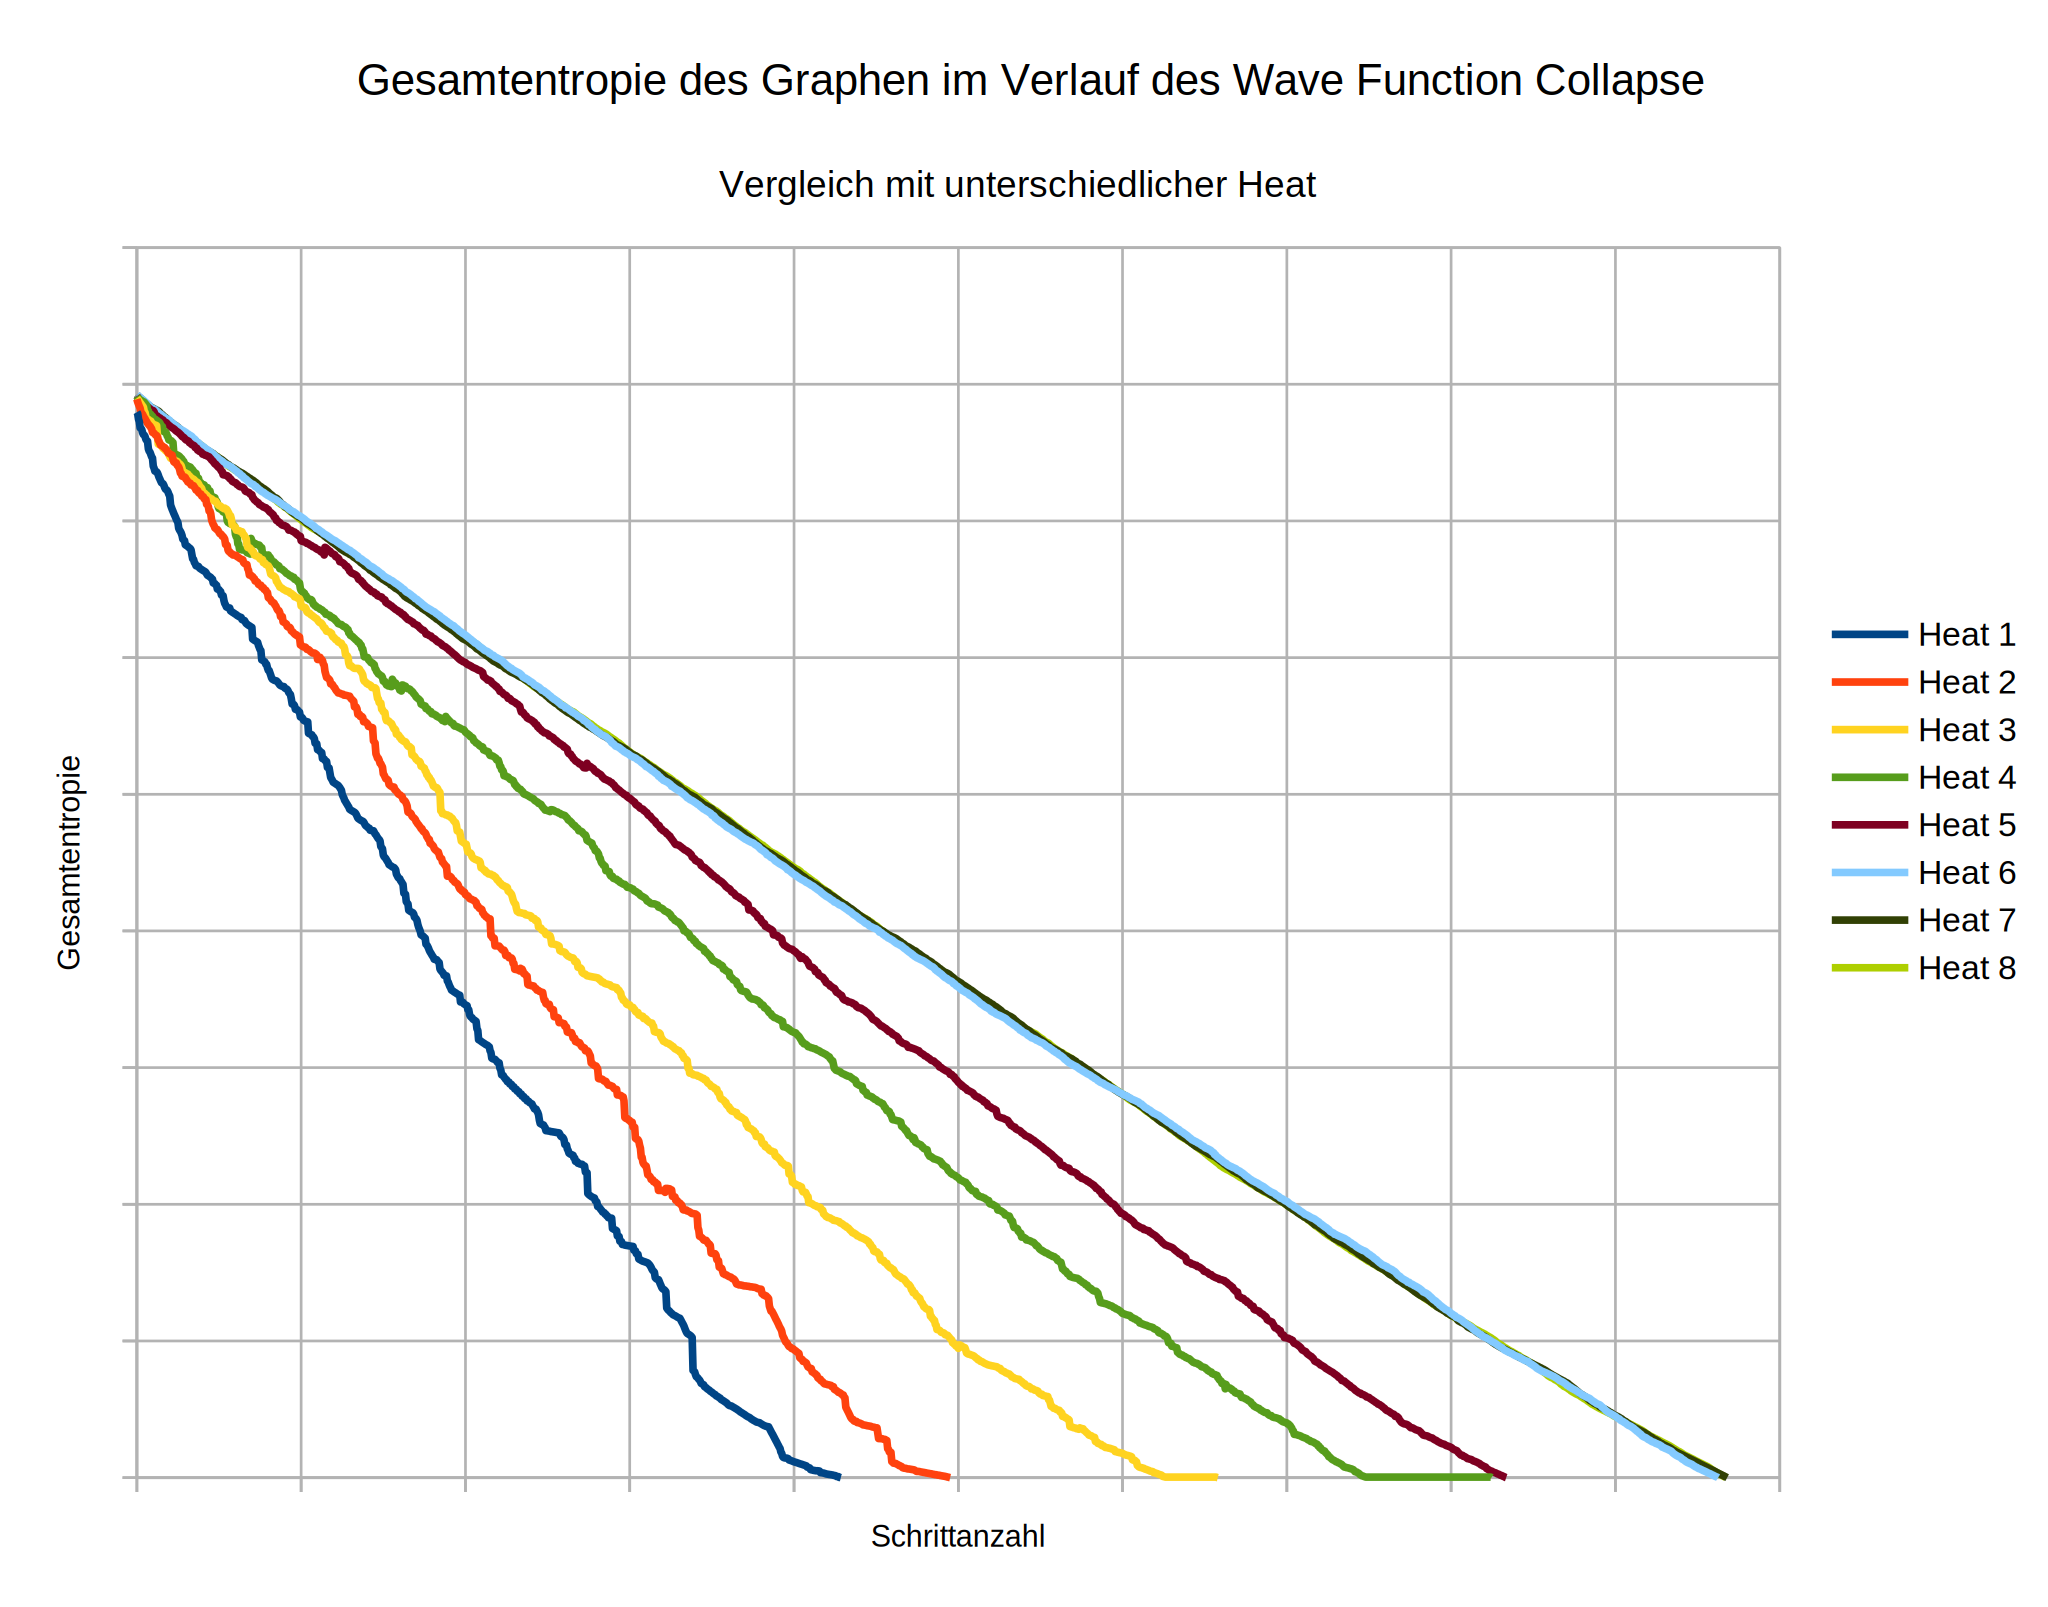
\includegraphics[width=\linewidth]{data/townscaper_grid/1.png} \caption{} \end{subfigure}
    \begin{subfigure}{0.18\textwidth} \includegraphics[width=\linewidth]{data/townscaper_grid/2.png} \caption{} \end{subfigure}
    \begin{subfigure}{0.18\textwidth} \includegraphics[width=\linewidth]{data/townscaper_grid/3.png} \caption{} \end{subfigure}
    \begin{subfigure}{0.18\textwidth} \includegraphics[width=\linewidth]{data/townscaper_grid/4.png} \caption{} \end{subfigure}
    \begin{subfigure}{0.18\textwidth} \includegraphics[width=\linewidth]{data/townscaper_grid/5.png} \caption{} \end{subfigure}
    
    \caption{
        Generierung eines Teils des Gitters für Townscaper \cite{stalberg_grid}. (a) Punkte werden generiert. (b) Triangulierung. (c) Kanten werden gelöscht, so dass Vierecke entstehen. (d) die Vierecke werden geviertelt. (e) Position der Knoten wird aufgelockert, so dass die Winkel zwischen Kanten gleichmäßiger sind.
    }
    \label{fig:townscaper_grid}
\end{figure}






\chapter{Wave Function Collapse auf Graphen}
    In diesem Abschnitt wir dargestellt wie der Wave Function Collapse Algorithmus erweitert wird, so dass die Ausgabe nicht nur auf einem Gitter von Zellen geschehen kann, sondern auch auf Zellen mit freier Anordnung und Verteilung, einem Graphen, arbeiten kann. Es wird erklärt welche Aspekt des Algorithmus angepasst werden und welche beibehalten werden können. Desweiteren wird ein neues Konzept names \textit{Heat} eingeführt, welches dem Nutzer erlaubt die erzielte Ähnlichkeit zum Beispiel zu verringern um die Erfolgschance des Algorithmus zu verbessern.
    
    
    \section{Beschränkung des Algorithmus und Idee zur Erweiterung}
        Die ursprüngliche Form des Wave Function Collapse nimmt ein 2D Pixelmuster oder Tilesets als Beispiel und produziert daraus wieder 2D Muster. 
        Pixel liegen stets auf einem quadratischen Gitter. Bei Tilesets ist die grafische Gestaltung des Tiles zwar uneingeschränkt, dennoch sind die Tiles selbst quadratisch. Dies schränkt die Gestaltung des Inhalts der Tiles in sofern ein, dass die Kanten zu anderen Kanten passen müssen. Auch bei 3D Beispielen werden die Modelle in blockförmige Bauteile zerschnitten, damit der Algorithmus auf einem 3D Gitter von Würfeln arbeiten kann.
        
        Solche Gitter bringen bestimmte Vorteile durch ihre Struktur mit sich. Die Benachbarung von Zellen ist implizit aus dem Gitter erkennbar, die Nachbarzellen befinden sich stets in festen Abständen in die vier Himmelsrichtungen im 2D Gitter und entlang der drei Achsen, also 6 Richtungen, im 3D Gitter. Die Überlappungsregeln aus dem Beispiel können also direkt von dem einem Gitter auf das andere übertragen werden. Der Nachteil solcher Gitter ist, dass die Ausgabe, im Ganzen, Artefakte des Gitter aufweist. Nur vertikale und horizontale Linien können im Pixelgitter exakt dargestellt werden, frei geformte Kurven oder organische Strukturen lassen sich nur durch Annäherung darstellen und es kann zu Aliasing kommen.
        
        \at{@placement und @flow}
        Im Kern des Wave Function Collapse wird geprüft, dass nur Zustände gewählt werden, die mit der Ausgabe bis dahin überlappen könnten. Die möglichen Überlappungen hängen dabei von der Richtung zwischen den Zellen ab. In einem Gitter kann jede Richtung zu einer Nachbarzelle aus dem Beispiel extrahiert werden. Wird die Anordnung und Benachbarung der Zellen nun aber vom Gitter gelöst, so ist es nicht mehr garantiert, dass die Richtungen zwischen Nachbarzellen auch im Beispiel existieren, stattdessen muss eine Funktion zur Übersetzung der tatsächlichen Richtung zu einer der extrahierbaren Richtungen definiert werden. Danach kann der Algorithmus wie zuvor mit den Überlappungen arbeiten um nun den Graphen zu befüllen.
    
    
    \section{Von Gittern zu Graphen}
        Ursprünglich arbeit Wave Function Collapse nur auf Gittern \cite{merrel} \cite{gumin}. Der Schritt zum Graphen als Fundament für die Ausgabe des Algorithmus ist sinnvoll \at{@wording}, da Gitter eine spezielle Art von Graphen darstellen. In dem Umfang dieser Arbeit werden aber auch nicht alle Arten von Graphen betrachtet, meistens ist die freie Anordnung und Verbindung von Knoten nicht notwendig. Da jede Kanten eines Gitters zuvor eine lokale Benachbarung dargestellt haben und die Regelextrahierung nur lokal arbeitet, beschränkt sich diese Arbeit nur auf Graphen in denen Kanten auch primär einen Knotenpunkt mit den Knotenpunkten in einem lokalen Umfeld verbindet. \at{@visual Gitter und Graph des Gitters} Der Algorithmus kann auch auf anderen Arten von Graphen angewendet werden, doch können daraus neue oder unerwartete Effekte hervortreten, die wiederum anderen Lösungswege benötigen.
        
        Ein Gitter bringt mit sich Information über Benachbarung und Position jeder Zelle die nun auf einem Graphen explizit angegeben werden müssen. Je nach Anordnung kann nun nicht nur die Richtung zur Nachbarzelle sondern auch deren Abstand und die Anzahl an Nachbarzellen variieren. Bevor der Algorithmus eine Ausgabe generieren kann, müssen diese Information vom Nutzer angegeben werden. \at{@wording explizit vs. implizit}
        
        \at{@placement @flow Lösungsraum undefiniert}
        Jede Kante des Graphen stellt eine Beschränkung des Lösungsraums dar. Bei einem Gitter ist jede Zelle, mit Ausnahme der Zellen am Rand, gleichermaßen beschränkt, jedoch kann die Anordnung des Graphen dazu führen dass einzelne Zelle weniger und andere stärker eingeschränkt werden. Eine Zelle mit zehn Nachbarn muss in einen Zustand collapsen, welcher zu den Zuständen der zehn Nachbaren passt. Ein Graph kann somit stark beschränkte und schwach beschränkte Regionen enthalten, während dass Gitter uniforme Beschränkung auf Zellen ergibt. Zur Erinnerung: es muss nur eine Zelle eine Widerspruch verursachen damit der Algorithmus fehlschlägt. Also sind solche Regionen starker Beschränkung besonderns entscheident für die Chance eine valide Ausgabe zu generieren, weil hier der Lösungsraum am kleinsten ist.
        
        \at{@incomplete Entropie erwähnen und für Regionen mit einer Grafik von der App darstellen}
    
    
        
    \section{Heat}
        In einem 2D Gitter sind die Nachbarn jeder Zelle per Definition in festen Richtungen und Abständen zu finden. Bei Graphen ist diese Anordnung frei. Während des Algorithmus werden die möglichen Zustände von Nachbarzellen auf Überlappung geprüft. Ein Zustand einer Zelle ist möglich, wenn er mit mindestens einem Zustand jeder Nachbarzelle überlappen kann. Die Überlappung zweier Zustände hängt von der Richtung zwischen den Umfeldern der Zustände abhängt ab. Das heißt, dass für den Nachbar im Norden einer Zelle nur die Überlappung der Zustände im Norden relevant ist. Die Richtung zu einer Nachbarzelle auf einem Graphen wird als der Vektor vom Mittelpunkt der Zelle zum Mittelpunkt der Nachbarzelle definiert. Der wichtigste Unterschied ist, dass die Richtung nun nicht mehr, wie auf dem Gitter, auf die Himmelsrichtungen beschränkt ist. 
        
        Es ist nicht möglich Regeln für eine beliebige Richtung aus dem Beispiel zu extrahieren, da jeder Pixel nur 8 angrenzende Pixel hat. Sieht man das Beispiel als eine Funktion an, so ist diese nicht an allen Punkten definiert. Man könnte durch Interpolation einen Mittelwert zwischen Pixeln berechnen, wenn das Bild eine kontinuierliche Funktion approximiert. Handelt es sich aber tatsächlich um eine diskrete Funktion, könnte eine Interpolation Werte ergeben die nicht Teil des Wertebereichs waren, in anderen Worten würde man Farbwerte erhalten die vorher nicht im Bild waren. Da die Ausgabe dem Beispiel ähnlich seien muss, entfällt diese Option.
        
        Es bleibt also nur die Möglichkeit, dass der tatsächlichen Richtung eine der messbaren Himmelsrichtungen zugewiesen wird. Hierfür wird die Kosinus-Ähnlichkeit \cite{cosine} \ref{fig:cosine} berechnet. Ist der Wert hoch, so zeigen die Vektoren in eine ähnliche Richtung, während entgegengesetze Vektoren eine geringe Ähnlichkeit haben. Es wird die Himmelsrichtung mit der höchsten Ähnlichkeit gewählt. 
        
        \begin{figure}[H]
    \centering
    
    $$ \mathrm{similarity}(\mathbf{a},\mathbf{b}) = \frac{\mathbf{a}\cdot\mathbf{b}}{\|\mathbf{a}\|_2\,\|\mathbf{b}\|_2} $$
    
    \caption{Formel für die Kosinus-Ähnlichkeit}
    
    \label{fig:cosine}
\end{figure}
        
        Nun kann mit dieser Auswahlt weitergearbeitet werden. Der Nachbar wird als in dieser Himmelrichtung liegend behandelt und daraus ergibt sich, welche Überlappungsregeln benutzt werden. Sind die Zellen beinahe oder ausschließlich entlang der Himmelrichtungen angeordnet, dann funktioniert diese Rundung gut. Liegt eine Nachbarrichtung nun aber genau zwischen zwei Himmelrichtungen, so haben beide die gleiche Ähnlichkeit und der Algorithmus muss willkürlich eine der beiden wählen. Diese Entscheidung wird bereits vor Beginn der Generierung getroffen, was den schlechtesten Zeitpunkt dafür darstellt, da am wenigsten Information vorliegt. Um zu wissen welche Himmelrichtung bessere Ergebnisse liefert, müssten beide Optionen jeweils ausprobiert und verglichen werden. Da jede Zelle mit ihrem finalen Zustand aber jede andere Zelle beeinflussen kann, müsste jede Kombination für alle Zellen geprüft werden, was schnell unmöglich wird. Stattdessen wäre es besser die Entscheidung bis zum letzten Moment, also dann wenn eine Zelle collapst wird, aufzuschieben. Zu diesem Zeitpunkt hat der Algorithmus die meisten Informationen und kann dadurch einen Widerspruch besser vermeiden. Beim collapsen wird der Zelle immernoch ein einziger Zustand zugewiesen, wodurch implizit ebend die Himmelsrichtung, mit der der gewählte Zustand mit den Nachbarzellen überlappt, ausgewählt wird.
        \\
        \\
        \textit{Heat} gibt an wie viele Himmelrichtungen der Algorithmus für Nachbarn betrachtet. Diese wird im Umfang dieser Arbeit für alle Zellen des Graphen einheitlich gesetzt und vor Beginn der Generierung festgelegt. Damit ein Zustand nun für eine Zelle möglich ist, muss dieser mit den Zuständen der Nachbarzellen überlappen. Nun muss die Überlappung entsprechend der Heat nicht nur noch entlang einer Himmelrichtung sein, sondern es können mehrere geprüft werden, wobei es reicht wenn eine der Himmelsrichtungen eine passende Regel hat. Ein Effekt höherer Heat ist, dass Zellen mehr mögliche Zustände haben, da es für jeden Zustand mehr passende Regeln gibt; die Entropie der Zellen ist tendenziell höher als bei geringer Heat.
        
        Die Anzahl der extrahierten Himmelsrichtungen begrenzt den Wertebereich für die Heat. Jeder Benachbarung kann minimal eine und maximal alle Himmelsrichtungen zugewiesen werden. Da Wave Function Collapse zuvor auf Gittern lief, konnten die Regelextraktion optimiert werden. Die reguläre Struktur des Gitters führt dazu, dass wenn für eine Zelle $A$ der Nachbar von $A$ im Norden($A_n$) passt und der Nachbar im Westen von $A_n$ passt, dann muss auch der Nachbar von $A$ im Nordwesten passen. Somit mussten nur die Überlappungsregeln für Norden, Süden, Westen und Osten gespeichert werden. Für die Generierung auf Graphen entfällt dies. Die diagonalen Himmelsrichtungen werden explizit gespeichert und behandelt.
    
    
    
    \section{Überblick}
        Ziel dieser Arbeit ist, die Generierung des Wave Function Collapse Algorithmus auf Graphen geschehen zu lassen. Hierfür wurden drei Anpassungen dargestellt:
        \begin{enumerate}
            \item Ein Gitter gibt implizit an, wo Zellen liegen und welche Zellen benachbart sind. Diese Informationen müssen im Graphen explizit gespeichert werden. 
            \item Für Gitter genügt es bei der Regelextraktion die Himmelrichtungen entlang der Achsen zu betrachtet. Bei Graphen sollten aber auch die Diagonalen extrahiert und gespeichert werden.
            \item Die aus dem Beispiel extrahierten Überlappungsregeln können nicht wie bei Gittern direkt angewendet werden. Die für eine Nachbarzelle relevanten Regeln werden aus der tatsächlichen Richtung zu dieser berechnet. Diese Zuweisung wird mittels Heat erweitert, so dass mehr als eine Himmelsrichtung ausgewählt werden kann.
        \end{enumerate} 



\chapter{Umsetzung}
    \at{@incomplete Einleitender Satz, was zur App sagen}
    
    \section{Generierung von Graphen}
        Die Graphen auf denen der Wave Function Collapse arbeiten soll, werden in dieser Arbeit mit dem folgenden Algorithmus generiert \ref{fig:graph_gen}. Der Algorithmus nimmt als Eingabe eine Menge an Punkten, welche die Knotenpunkte des Graphen werden. Aus den Punkten wird eine Delaunay-Triangulierung erstellt. Hierfür wird er Boywer-Watson Algorithmus \cite{bowyer, watson} verwendet. Danach wird das Voronoi-Diagramm zu der Triangulierung gefunden. Der duale Graph der Delaunay-Triangulierung ist das Voronoi-Diagramm \at{@visual}, d.h. jeder Knotenpunkt des Voronoi-Diagramms entspricht einer Fläche der Triangulierung und jede Fläche im Voronoi-Diagramm entspricht einem Knotenpunkt in der Triangulierung. Die Kanten der Dreiecke geben an, welche Zellen aneinander angrenzen, während die Voronoi-Zellen die Form einer Zelle für die Darstellung geben. In Abbildung \ref{fig:graph_examples} sind einige Beispiele von generierten Graphen dargestellt. Es ist zuerkennen, dass regelmäßige Gitter nur eine spezielle Form von Graphen darstellen. 
        
        \at{@citation delaunay und voronoi, wenn nicht schon vorher passiert ist.}
        \at{@visual für Boywer-Watson algorithmus}
        
        \begin{algorithm}
    \caption{Generierung eines Graphen}
    \label{alg:graph_gen}
        
    \begin{enumerate}
    \item Erstelle eine Menge an Punkten
    
    \item Generiere die Delaunay-Triangulierung der Punkte
    \subitem Die Ecken und Kanten aller Dreiecke bilden den Graphen
        
    \item Erstelle die Voronoi-Zellen aus der Triangulierung \begin{enumerate}
        \item Finde alle Dreiecke, die einen Punkt teilen
        \item Die Schwerpunkte dieser Dreiecke sind die Eckpunkte der Zelle
        \item Verbinde die Eckpunkte der Zelle mit Kanten
        \item Begrenze die Voronoi-Zellen auf den gewünschten Bereich 
        \subitem siehe Abbildung \ref{fig:voronoi_clipping}
        \end{enumerate}
    \end{enumerate}
        
\end{algorithm}
        \begin{figure}[H]
    \centering
    \begin{subfigure}{0.18\textwidth} 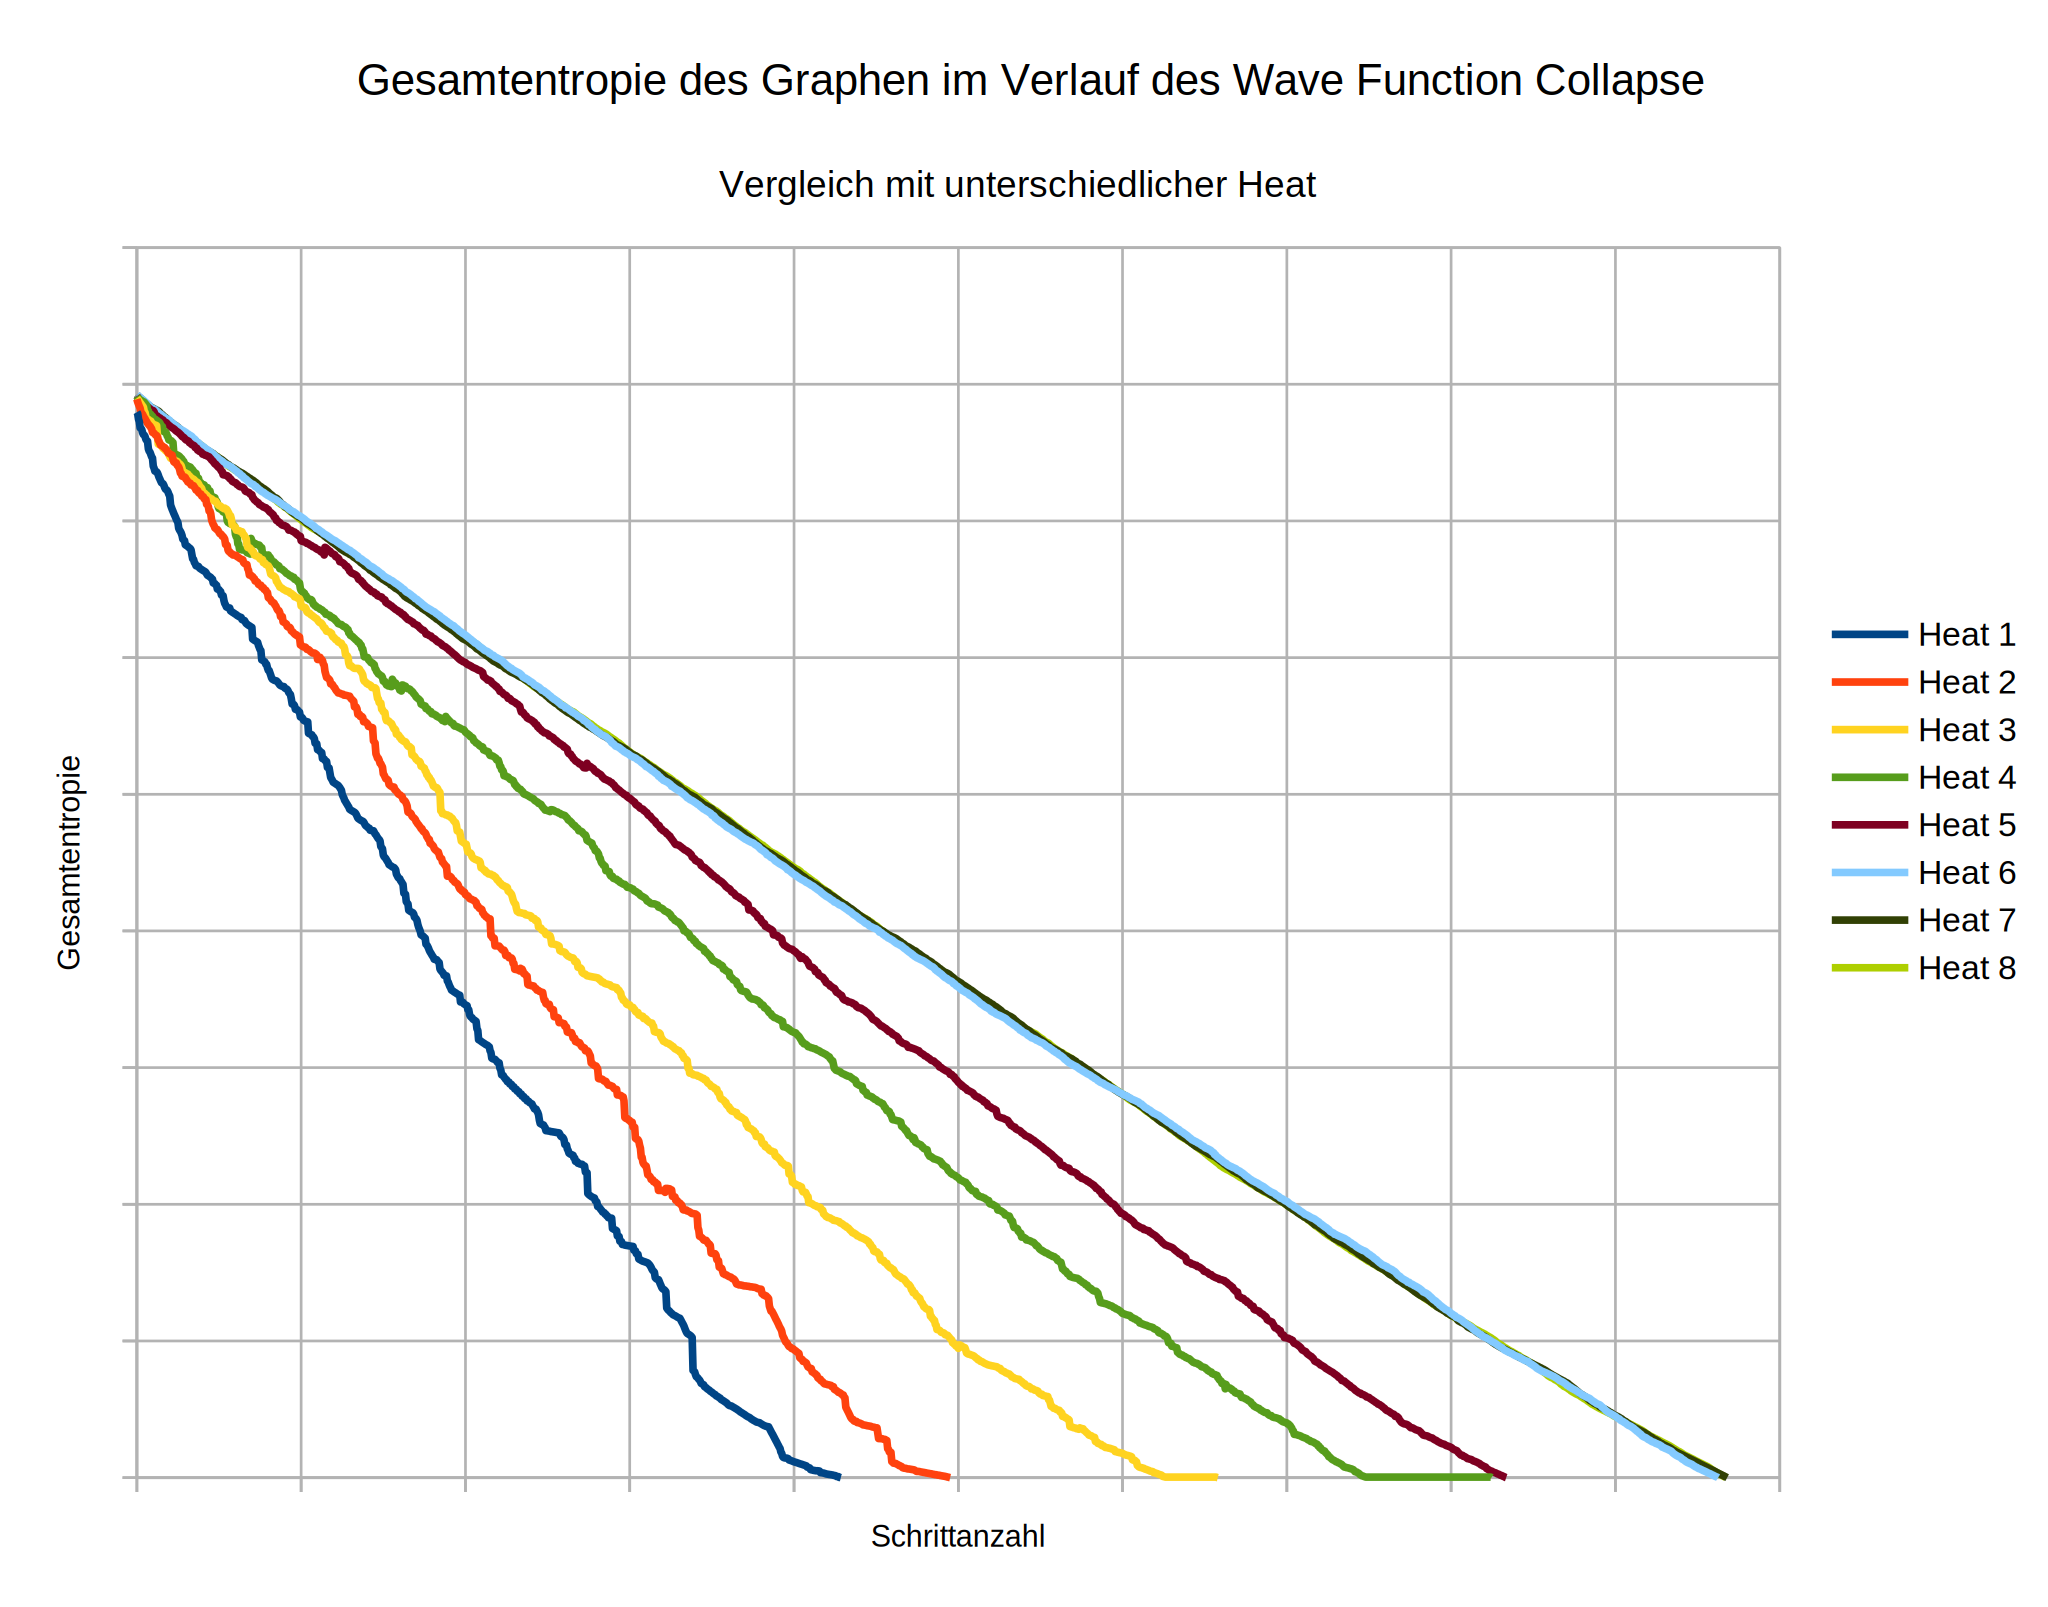
\includegraphics[width=\linewidth]{data/townscaper_grid/1.png} \caption{} \end{subfigure}
    \begin{subfigure}{0.18\textwidth} \includegraphics[width=\linewidth]{data/townscaper_grid/2.png} \caption{} \end{subfigure}
    \begin{subfigure}{0.18\textwidth} \includegraphics[width=\linewidth]{data/townscaper_grid/3.png} \caption{} \end{subfigure}
    \begin{subfigure}{0.18\textwidth} \includegraphics[width=\linewidth]{data/townscaper_grid/4.png} \caption{} \end{subfigure}
    \begin{subfigure}{0.18\textwidth} \includegraphics[width=\linewidth]{data/townscaper_grid/5.png} \caption{} \end{subfigure}
    
    \caption{
        Generierung eines Teils des Gitters für Townscaper \cite{stalberg_grid}. (a) Punkte werden generiert. (b) Triangulierung. (c) Kanten werden gelöscht, so dass Vierecke entstehen. (d) die Vierecke werden geviertelt. (e) Position der Knoten wird aufgelockert, so dass die Winkel zwischen Kanten gleichmäßiger sind.
    }
    \label{fig:townscaper_grid}
\end{figure}
        
        \at{@incomplete was muss noch im text vorkommen? warum voronoi clipping}
        Es ist normal, dass ein solches Voronoi-Diagramm an den Rändern Zellen ergeben kann die auf einer Seite offen sind, weil die Kanten zwischen den Ecken der Zelle, den Umkreismittelpunkten, keinen Schnittpunkt haben. Ich habe mich dazu entschieden, bei solchen Zellen weitere Eckpunkte einzufügen, so dass das alle Zellen durch einen freigewählten rechteckigem Bereich begrenzt sind. Dafür prüfe ich ob ein Eckpunkt außerhalb des Bereichs liegt und finde dann den Schnittpunkt von der Kante zu dem Eckpunkt mit dem Rechteck des Bereichs und ersetze den Eckpunkt mit diesem Schnittpunkt. Dieser Schritt passiert so lange bis alle Eckpunkte innerhalb oder auf dem Rand des Bereichs liegen.
            Siehe Abbildung \ref{fig:voronoi_clipping}.

        \begin{figure}[H]
    \centering
    \begin{subfigure}{0.18\textwidth} 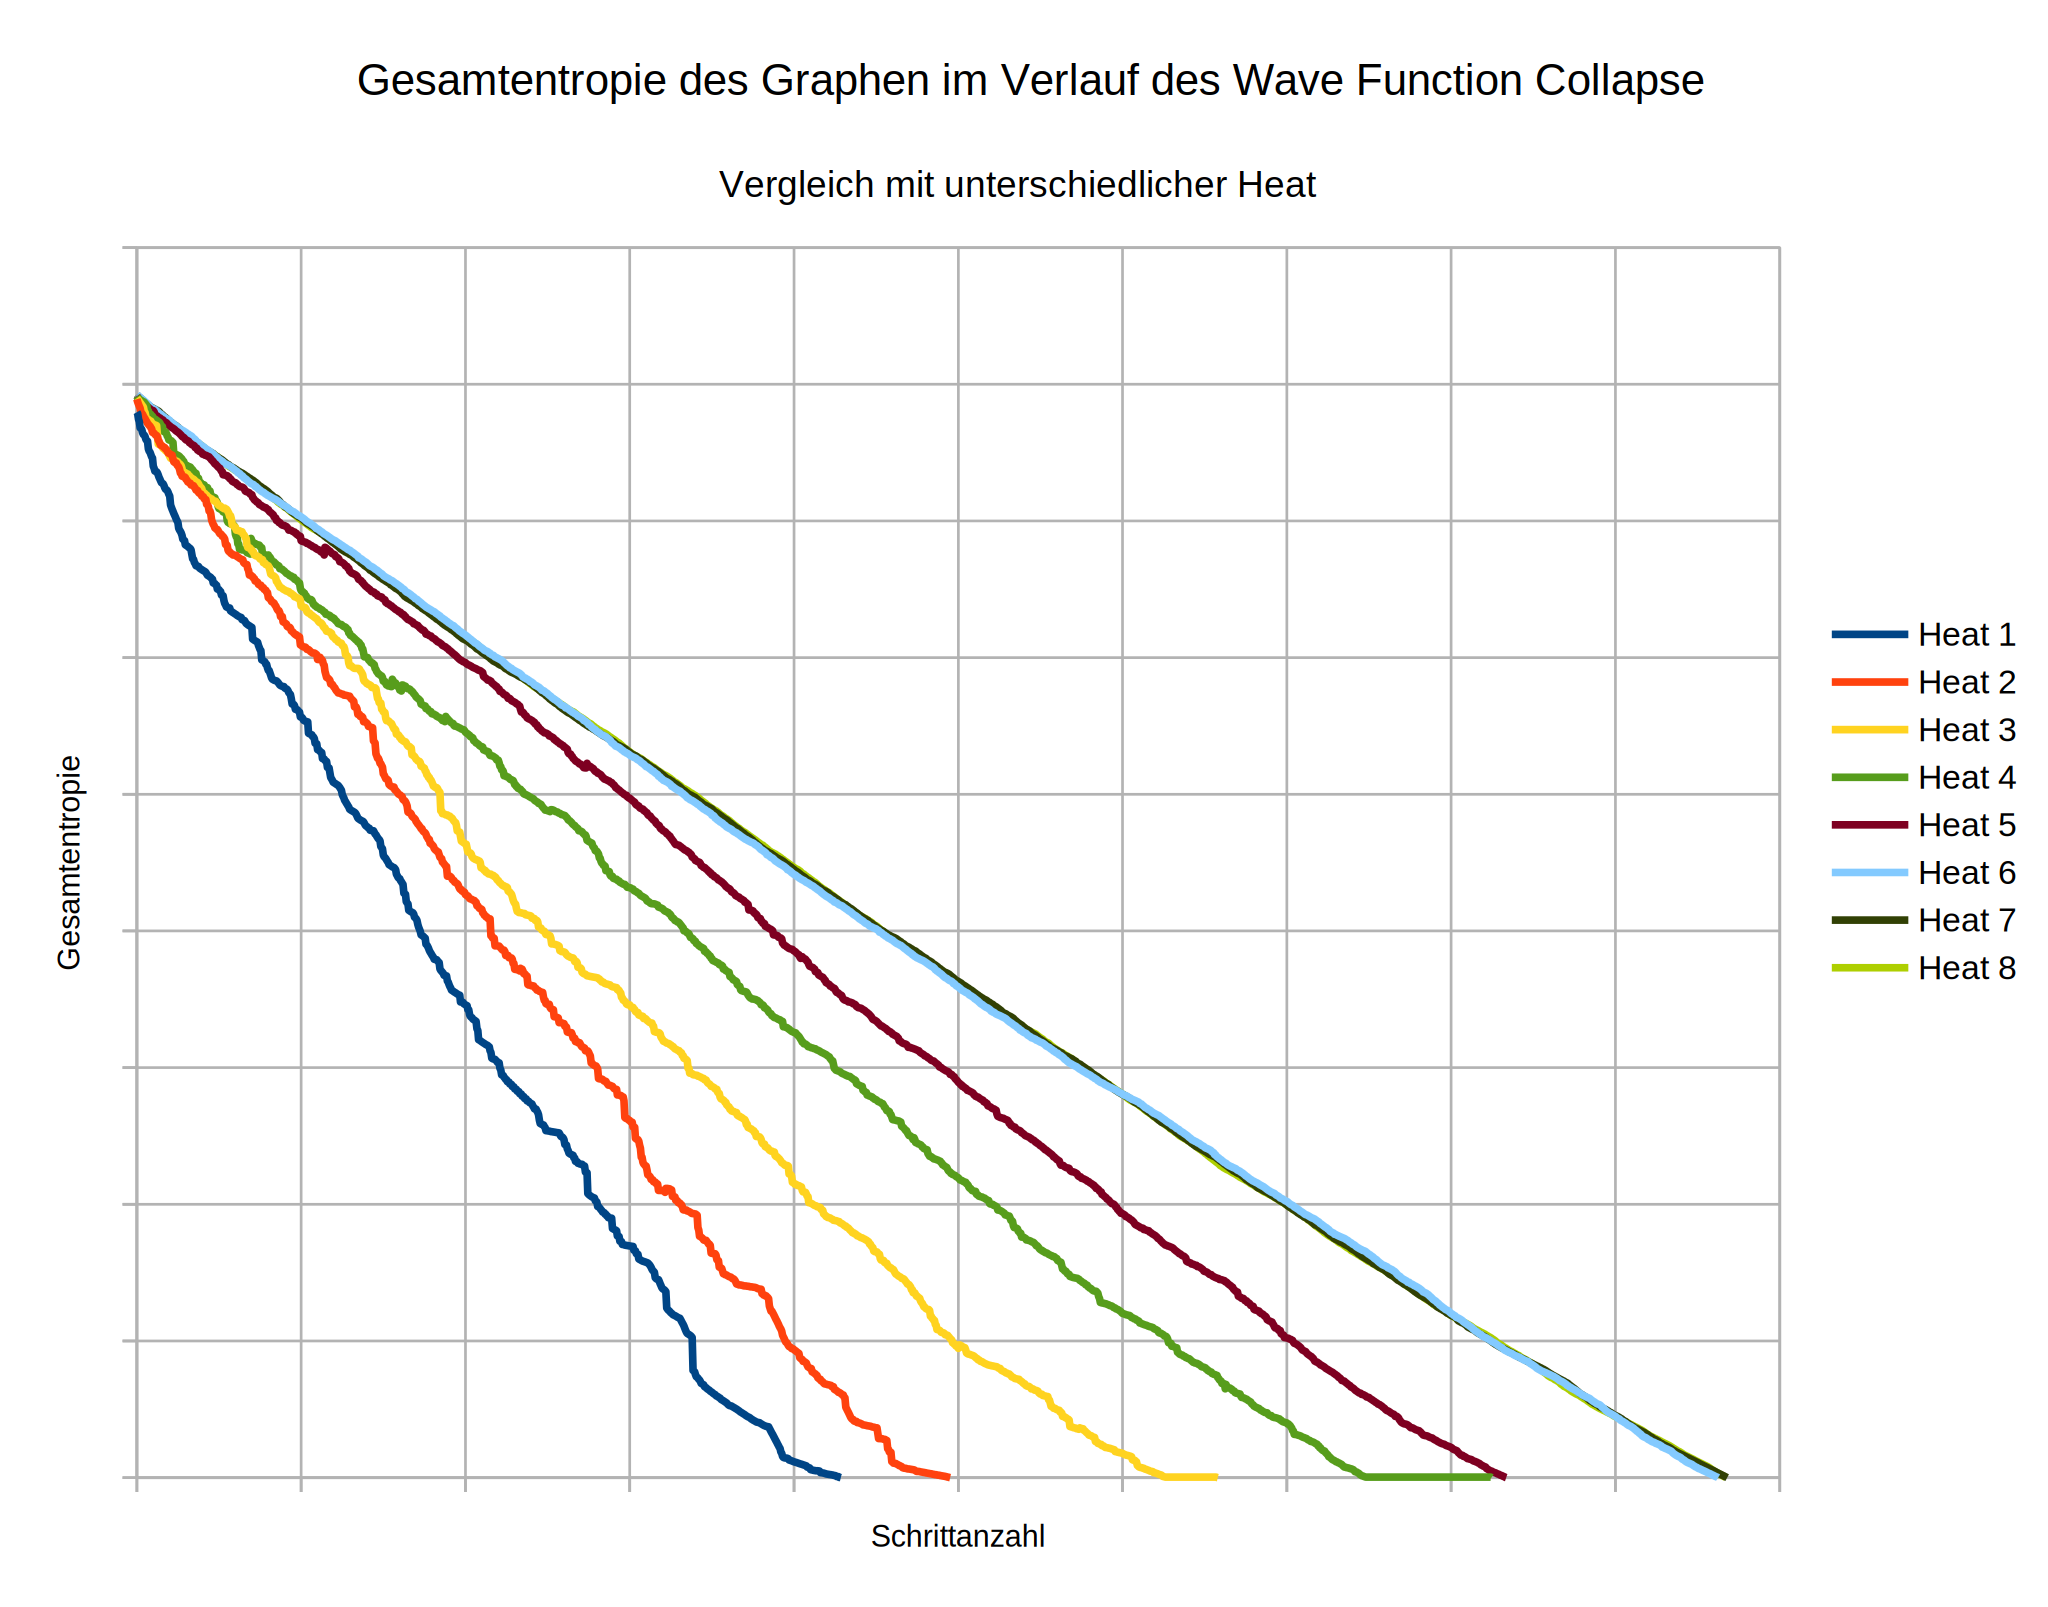
\includegraphics[width=\linewidth]{data/townscaper_grid/1.png} \caption{} \end{subfigure}
    \begin{subfigure}{0.18\textwidth} \includegraphics[width=\linewidth]{data/townscaper_grid/2.png} \caption{} \end{subfigure}
    \begin{subfigure}{0.18\textwidth} \includegraphics[width=\linewidth]{data/townscaper_grid/3.png} \caption{} \end{subfigure}
    \begin{subfigure}{0.18\textwidth} \includegraphics[width=\linewidth]{data/townscaper_grid/4.png} \caption{} \end{subfigure}
    \begin{subfigure}{0.18\textwidth} \includegraphics[width=\linewidth]{data/townscaper_grid/5.png} \caption{} \end{subfigure}
    
    \caption{
        Generierung eines Teils des Gitters für Townscaper \cite{stalberg_grid}. (a) Punkte werden generiert. (b) Triangulierung. (c) Kanten werden gelöscht, so dass Vierecke entstehen. (d) die Vierecke werden geviertelt. (e) Position der Knoten wird aufgelockert, so dass die Winkel zwischen Kanten gleichmäßiger sind.
    }
    \label{fig:townscaper_grid}
\end{figure}
    
    
    \section{Phasen \at{@naming}}
        \at{@placement Phasen und Backtracking gehören zusammen sonst gibt es keinen Grund das hier so aufzudröseln}
        \at{@incomplete Schritt als global und festen Begriff im Algorithmus darstellen}
        Der Algorithmus \ref{fig:wfc_back} generiert die Ausgabe schrittweise. Ein Schritt kann in vier Phasen geteilt werden: Search, Pick, Observe und Propagate.
        
        \begin{figure}[H]
    \centering
    \begin{minipage}{\linewidth}
        \rule{\linewidth}{0.4pt}
        
        \begin{enumerate}
            \item Führe den nächsten \textbf{Schritt} aus: \begin{enumerate}
                \item \textbf{Search}: Finde die Zellen mit der geringsten Entropie \begin{enumerate}
                    \item Sind alle Zellen kollabiert? $\rightarrow$ \textbf{Done}
                    \item Erstelle ein Liste der gefundenen Zellen
                \end{enumerate}
                
                \item \textbf{Pick}: Wähle eine Zelle aus \begin{enumerate}
                    \item Ist die Liste der Zellen leer? $\rightarrow$ \textbf{Backtrack}
                    \item Entferne die gewählte Zelle aus der Liste
                    \item Notiere alle möglichen Zustände der Zelle in einer Liste
                \end{enumerate}
                
                \item \textbf{Observe}: Wähle einen Zustand aus \begin{enumerate}
                    \item Entferne den gewählten Zustand aus der Liste
                    \item Kollabier die Zelle in den Zustand
                    \item Ist die Liste der Zustände leer? $\rightarrow$ \textbf{Backtrack}
                \end{enumerate}
                
                \item \textbf{Propagate}: Prüfe alle Nachbarn von geänderten Zellen \begin{enumerate}
                    \item Erstelle eine Liste zu prüfender Zellen
                    \item Füge die ausgewählte Zelle ein
                    \item Prüfe alle Nachbarzellen ob ihre Zustände noch passen
                    \item Füge die Nachbarn in die Liste ein, wenn sie sich verändert haben
                    \item Hat die Nachbarzelle keine möglichen Zustände mehr? $\rightarrow$ \textbf{Backtrack}
                \end{enumerate}
                
                \item Geh zum nächsten \textbf{Schritt}
            \end{enumerate}
            \item \textbf{Backtrack}: \begin{enumerate}
                \item Gehe zum gewünschten Schritt zurück
                \item Gehe eine Phase in dem Schritt zurück
                \item Füge alle Zustände aller Zellen, dessen Entfernungsschritt nun nach dem aktuellen Schritt liegt, wieder in die Zelle ein
            \end{enumerate}
            \item \textbf{Done}: Gib das Resultat aus
        \end{enumerate}
            
        \rule{\linewidth}{0.4pt}
    \end{minipage}
    
    \caption{Wave Function Collapse mit Backtracking}
    
    \label{fig:wfc_back}
\end{figure} 
        
        Zu Beginn wird die Zelle mit der geringsten Entropie gesucht, die noch nicht collapsed ist. Die Entropie einer Zelle wird als die Shannon-Entropie \cite{shannon} der noch möglichen Zustände berechnet. Es ist möglich, dass mehrere Zellen die gleiche Entropie haben. Zum Beispiel sind alle Zellen am Anfang in der Superposition aller Zustände, wodurch alle Zellen die selbe Entropie haben. Aus der Menge an gefundenen Zellen wird in diesem Fall in der Pick-Phase eine Zelle zufällig ausgewählt.
        
        In der Observe-Phase wird ein Zustand aus der Superposition zufällig ausgewählt und die Zelle in diesen Zustand collapsed. Die anderen Zustände werden entfernt, was Einfluss auf die Nachbarzellen haben kann. Die Wahrscheinlichkeit eines Zustands, gewählt zu werden, hängt von dessen Häufigkeit im Beispiel ab. 
        
        Danach beginnt die Propagate-Phase. Eine Liste aller geänderten Zellen wird mit der observierten Zelle initialisiert. Jede Zelle in der Liste wird einzeln entfernt und wie folgt bearbeitet. Alle Nachbarzellen der betrachten Zellen prüfen, welche ihrer Zustände mit keinem der Zustände der betrachteten Zellen noch überlappen. Diese Zustände werden entfernt und jede Nachbarzelle die sich so verändert hat, wird der Liste angefügt. Sollte dabei auch der letzte mögliche Zustand einer Zelle unmöglich gewurden sein, so wurde ein Widerspruch erreicht; es kann nun keine Lösung mehr gefunden werden. Diese Phase dauert so lange, bis die Liste leer ist, sich also keine Zellen mehr verändern.
        
        
    \section{Backtracking}
        \at{@incomplete? wieso so und nicht simpler: kann nicht einfach zustand wieder einfügen und alle passenden zustände für nachbar einfügen, weil diese durch andere vielleicht doch unmöglich sind. dann muss alle prüfen (Propagate) aber rückwärts, oder alles speichern/kopie ist verschwenderisch, statt für jeden schritt alle zellen zu kopieren, kopieren wir für jede Zelle jeden schritt, dann fällt auf, dass nur der schritt an dem der Zustand entfernt wird relevant ist.}
        
        Wenn der Algorithmus einen Widerspruch entdeckt, muss nicht immer alle Arbeit verworfen werden. Gerade bei größeren oder komplizierteren Mustern oder Graphen ist es wahrscheinlich, dass beim ersten Versuch keine Lösung gefunden wird, weil die Komplexität den Lösungsraum stärker einschränkt. Wenn ein Widerspruch in einer Zelle aber nun nur von den direkten Nachbar abhängt, so ist es wahrscheinlich dass weiter entfernte bereits gelöste Zellen dennoch kompatibel sind. Um einen lokalen Widerspruch aufzulösen muss meistens nur lokal eine andere Entscheidung getroffen werden.
        
        Um Backtracking umzusetzen müssen mehr Informationen behalten werden als nur der Zustand des Gitters zum aktuellen Zeitpunkt. Will man nun wieder einen Schritt zurückgehen muss man wissen, welche Entscheidung man zuvor bereits getroffen hat um dessen Effekt rückgängig zu machen. Dabei genügt es nicht nur die collapste Zelle und den Zustand wieder zu entfernen, weil jede Zelle von mehreren Nachbarn beeinflusst wird. Die Zustandsmenge einer Zelle ist die Schnittmenge der möglichen Nachbarzuständen der Nachbar. Somit kann es sein, dass ein Zustand A aus der Menge wegen mehreren Einschränkungen von mehreren Nachbarn fehlt. Nimmt man nun durch Backtracking eine dieser Einschränkungen wieder zurück, so ist es nicht offensichtlich, ob Zustand A nun wieder möglich ist, ohne alle Einschränkungen auf die Zelle neu zu berechnen.
        Entweder man macht die Änderung nur lokal rückgängig und berechnet immer alle Zellen neu, bis sich keine mehr ändern. Oder man speichert ab, zu welchem Zeitpunkt ein Zustand unmöglich geworden ist und prüft ob dieser Zeitpunkt nach dem Schritt zurück weiterhin in der Vergangenheit oder nun in der Zukunft liegt\at{@wording visualisieren oder eine bessere Metapher finden}. Bei zweiterem müssen alle solche Zustände als wieder möglich betrachtet werden.
        Diese Art die Menge an Zuständen darzustellen ist okay \at{@wording}, weil sich für jede Zelle die Zustandsmenge in jedem Schritt des Algorithmus immer nur verkleinert oder gleichbleibt. Ist ein Zustand durch die Nachbar unmöglich so wird er auch nie wieder an späterem Zeitpunkt möglich.
        
        Desweiteren sollen bereits gemachte Entscheidungen, die zu einem Widerspruch führen, nicht noch einmal wiederholt werden. Die Entscheidungspunkte in der  Pick- und Observe-Phase können gleich behandelt werden. Wir können die List an Auswahlmöglichkeiten für später speichern und die ausgewählte Zelle oder den ausgewählten Zustand von der Liste entfernen. Wird auf einen Schritt gebacktrackt, so kann einfach die nächste Möglichkeit auswählt werden. Der Algorithmus läuft ab dann normal weiter .In der Umsetzung wird für jede Zelle eine Liste aller Zustände gespeichert. Jeder Zustand ist entweder möglich und wurde noch nicht entfernt oder ist unmöglich und speichert den Zeitpunkt an dem er unmöglich wurde. Hierbei ist der Zeitpunkt einfach die Nummer des Schritts an dem der Zustand unmöglich wurde. 
        
        \at{@placement}
        Der Algorithmus ist in Abbildung \ref{fig:wfc_back} dargestellt. Für jeden Schritt des Algorithmus wird auch die Liste der gefundenen Zellen in der Search-Phase gespeichert. Wenn in der Pick-Phase eine Zelle ausgewählt wird, wird diese aus der Liste entfernt, damit diese beim Backtracken nicht erneut gewählt wird. Ebenso werden in der Observe-Phase alle wählbaren Zustände gespeichert und mit jedem Lösungsversuch wird der gewählte Zustand entfernt. Nun wurde aber eine Schwachstelle in den Algorithmus eingeführt. Wenn zuvor in der Search-Phase keine Zellen in Superposition mehr gefunden wurden, bedeutete dies, dass alle Zellen tatsächlich collapsed waren. Nun kann es sein, dass alle Zellen, die gefunden wurden, zu einem Widerspruch führen würden und entfernt wurden. Somit würde keine Zelle mehr wählbar sein. Auch in der Observe-Phase war es zuvor unmöglich keinen Zustand mehr auswählen zu können, da eine Zelle mit leerer Zustandsmenge bereits zuvor als Widerspruch identifiziert wurden wäre. In diesen Fällen wurde ein Widerspruch erreicht und es muss zum Backtracking kommen. Schließlich wurden alle noch möglichen Entscheidungen bereits getroffen und ausgewertet und keine Lösung gefunden. Somit führt dieser Schritt zwar nicht direkt zu einem Widerspruch in einer Zelle, aber alle folgen Schritte werden irgendwann zu einem Widerspruch führen. Als Anmerkung: wird auf diese Weise bis zum ersten Schritt gebacktrackt und führen dann auch dort alle möglichen Entscheidungen zu einem Widerspruch, so kann die Kombination aus Beispiel und Graph keine Ausgabe ergeben.

        \at{@incomplete Datenstruktur der Regeln so dass es simpel mit mehr oder weniger Heat ist erklären}


\chapter{Ergebnisse und Diskussion}
    \at{@incomplete Einleitender Satz}
    
    \begin{itemize} % Ergebnisse
    \item Base Case - Gitter
    \item Bilder mit unterschiedlichen Graphen: Einfache, Komposition(vier in eins, außen und innen)
    \end{itemize}
    
    \begin{itemize} % Diskussion
    \item Vergleich zum WFC, wie und was vergleichen?
    \item Lokale Ähnlichkeit im Vergleich zum Input
    \item Linienmuster und Flächenmuster in Beispielen
    \end{itemize}
    
    \section{Der Effekt von Heat auf die Ausgabe}
        \at{@incomplete introduction}
        \\
        \\
        Abbildung \ref{fig:hex_heat} zeigt den Einfluss von Heat auf die Qualität der Ausgabe bei gleichem Beispiel und Graph. Das Beispiel kann auf dem Quadratgitter ohne weitere Probleme genutzt werden, während der Graph mit den Sechsecken bei geringer Heat uninteressante Ausgaben generiert. \at{@incomplete (a) erwähnen}
        
        \begin{figure}[H]
    \centering
    \begin{subfigure}{0.18\textwidth} 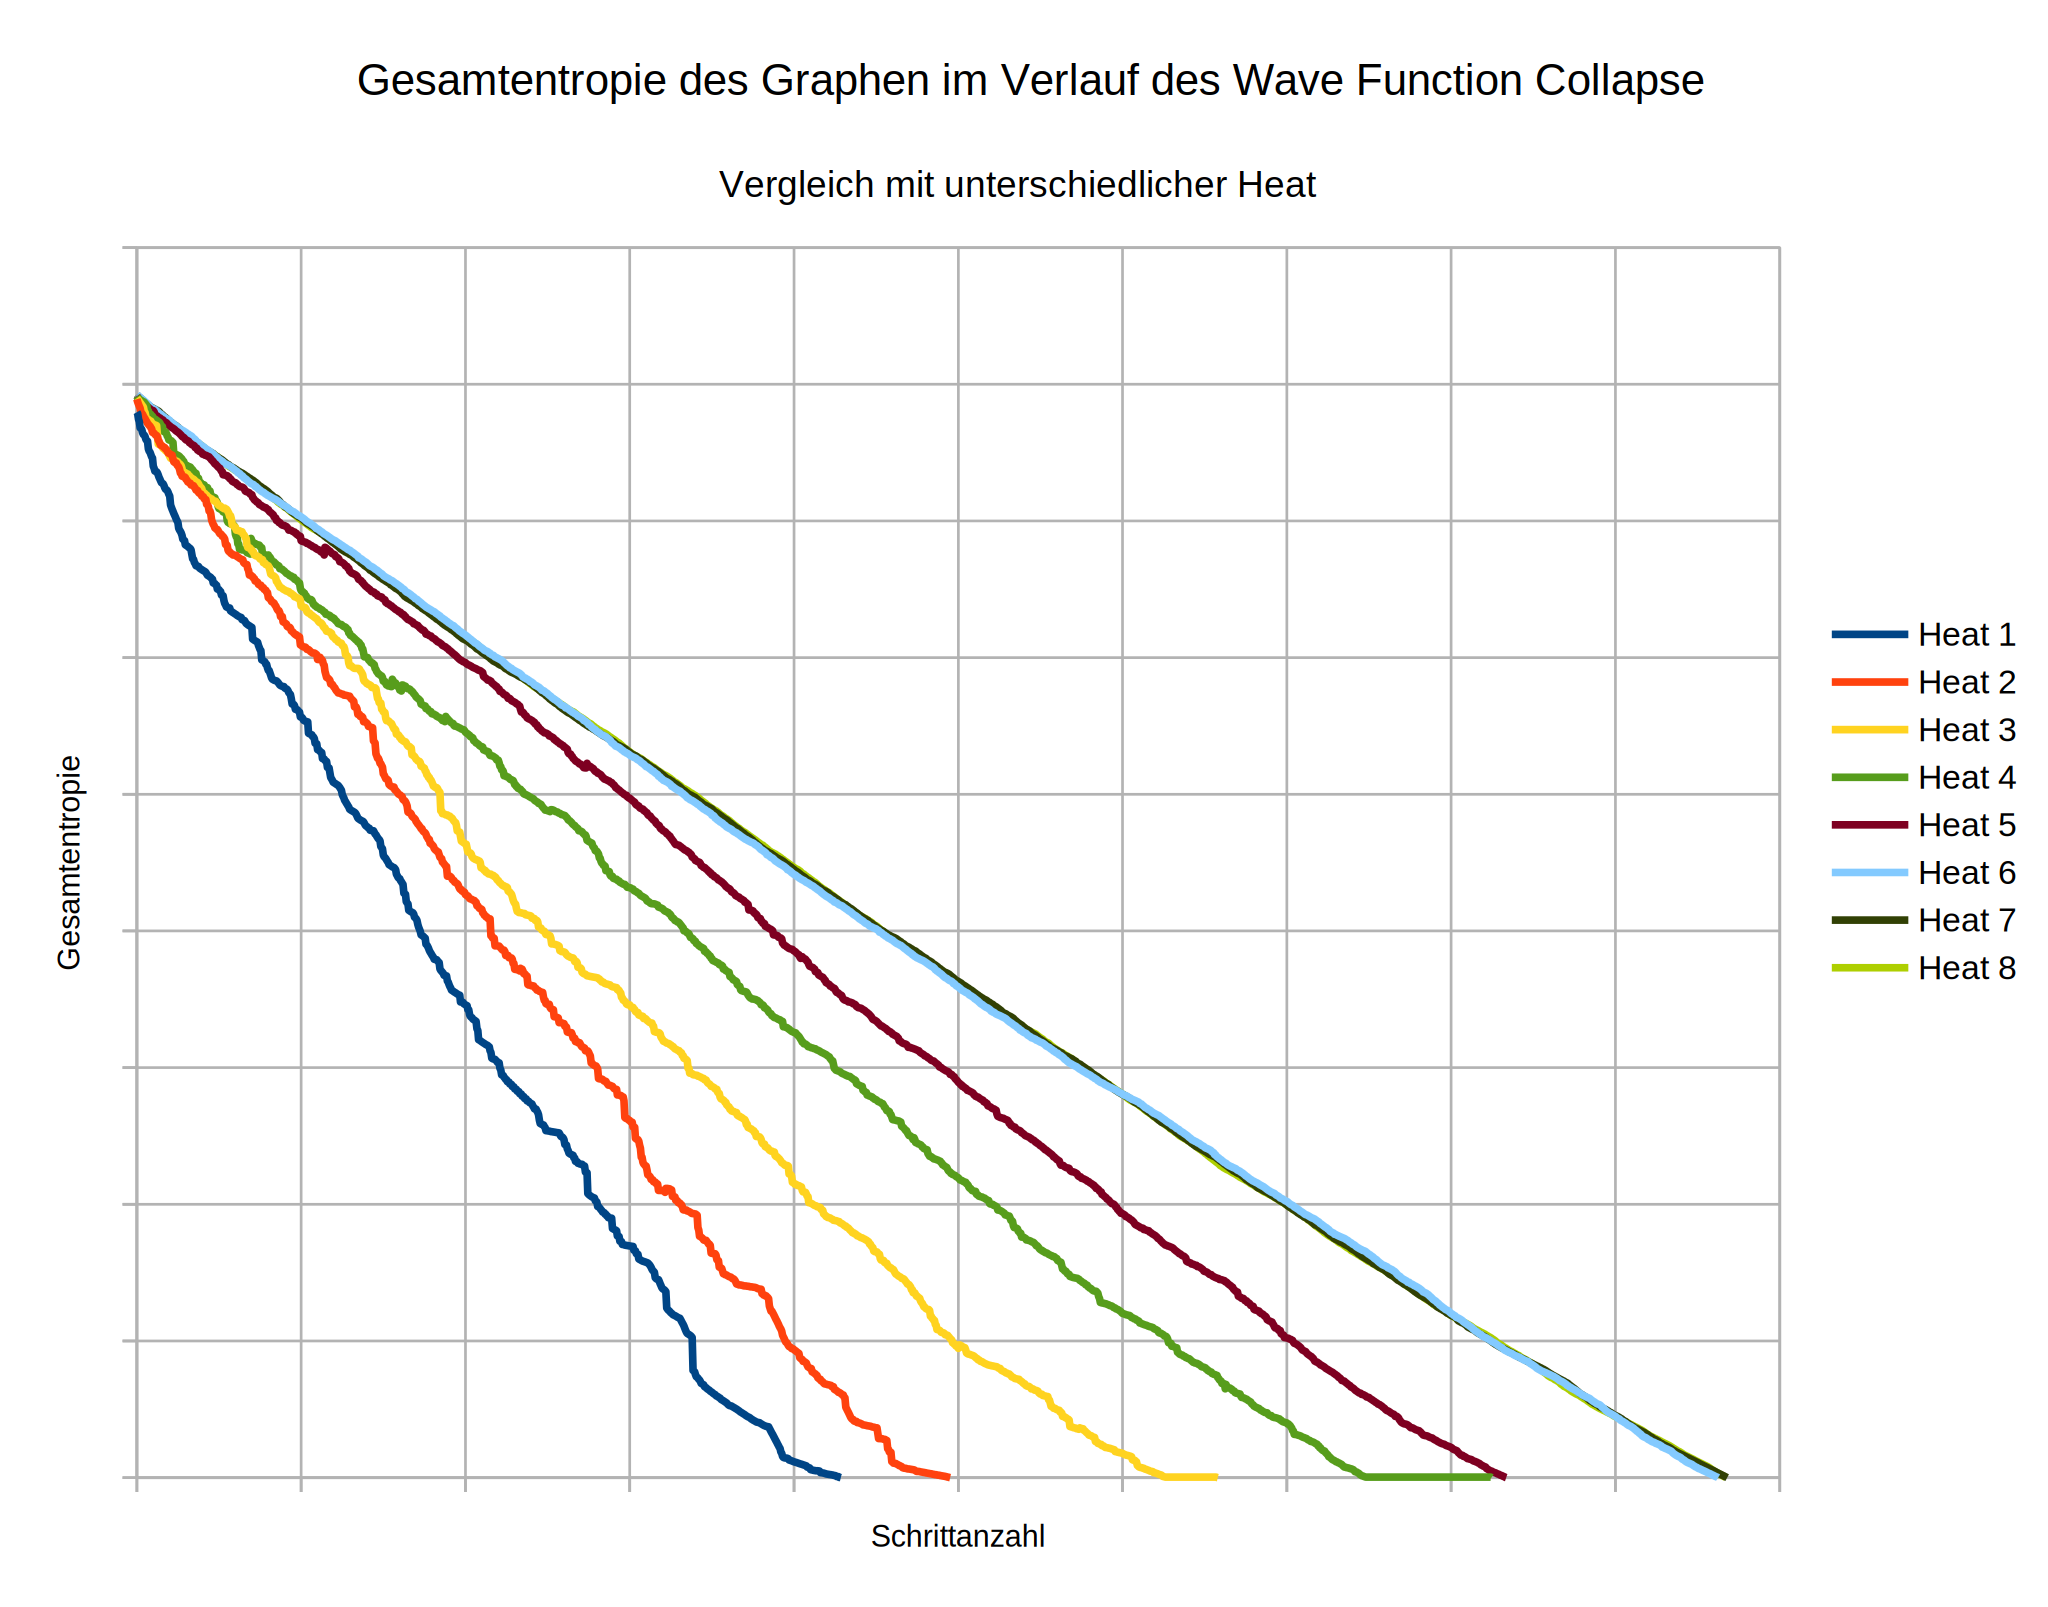
\includegraphics[width=\linewidth]{data/townscaper_grid/1.png} \caption{} \end{subfigure}
    \begin{subfigure}{0.18\textwidth} \includegraphics[width=\linewidth]{data/townscaper_grid/2.png} \caption{} \end{subfigure}
    \begin{subfigure}{0.18\textwidth} \includegraphics[width=\linewidth]{data/townscaper_grid/3.png} \caption{} \end{subfigure}
    \begin{subfigure}{0.18\textwidth} \includegraphics[width=\linewidth]{data/townscaper_grid/4.png} \caption{} \end{subfigure}
    \begin{subfigure}{0.18\textwidth} \includegraphics[width=\linewidth]{data/townscaper_grid/5.png} \caption{} \end{subfigure}
    
    \caption{
        Generierung eines Teils des Gitters für Townscaper \cite{stalberg_grid}. (a) Punkte werden generiert. (b) Triangulierung. (c) Kanten werden gelöscht, so dass Vierecke entstehen. (d) die Vierecke werden geviertelt. (e) Position der Knoten wird aufgelockert, so dass die Winkel zwischen Kanten gleichmäßiger sind.
    }
    \label{fig:townscaper_grid}
\end{figure}
        
        Eine intuitive Erklärung ist, dass die Linien im Beispiel stets nur eine Zelle breit sind. Im Graph können die horizontalen Linien generiert werden, weil die Sechsecke selbst horizontal in Reihen angeordnet sind, während es keine rein vertikalen Zellenspalten gibt. Jedes Sechseck hat zwei Nachbarzellen oberhalb und zwei unterhalb. Bei Heat=1 wird beiden Norden/Süden zugewiesen. Will der Algoritmus nun bei einer Zelle eine vertikalen Linie, also die Zustände die dieses Muster abbilden, platzieren, so müssen nun beide oberen Nachbarzellen auch eine Zustand, der eine vertikale Linie darstellt, erhalten. Hier kommt es zum Konflikt, da diese beiden Zellen horizontal in der gleichen Reihe liegen, es aber im Beispiel keine vertikalen Linien direkt nebeneinander gibt. Es kann also keine Zelle Teil einer vertikalen Linie sein. 
        
        Bei (c) können dennoch scheinbar vertikale Linien generiert werden, da nun die oberen Zellen jeweils als im Norden und imd Nordosten/-westen betrachtet werden. Ebenso können die horizontalen Nachbarn als im Westen oder im Süd-/Nord-westen behandelt werden. Soll eine Zelle nun Teil einer vertikalen Linie sein, kann nur eine der oberen Nachbarnzellen als im Norden behandelt werden und die andere als die jeweilige Diagonale. 
        
        Der Effekt von höherer Heat ist, das die Menge an möglichen Zuständen vergrößert wird, indem mehr Überlappungsregeln in Betracht gezogen werden. Dadurch ist es auch unwahrscheinlicher, dass für eine Zelle keine Zustände mehr möglich sind und ein Widerspruch entsteht. Gleichzeitig werden nun aber auch Ausgaben generiert, die eine tatsächlich geringere Ähnlickkeit zum Beispiel haben. So ist die Ausgabe in (b) zwar weniger interessant als die in (c), aber die horizontalen Linien und die grauen Flächen dazwischen passen exakt zur Teilen des Beispiels. Bei (c) werden auch vertikalen Linien generiert, aber diese haben knicke und sind eher zickzackartig als die Senkrechten des Beispiels. Eine Erhöhung der Heat verschlechtert die lokale Ähnlichkeit der Ausgabe zum Beispiel und verbessert die Wahrscheinlichkeit erfolgreich eine nicht triviale Lösung zu generieren.
        \\
        \\
        In Abbildung \ref{fig:heat_rotation} ist dargestellt, wie Heat auch als eine lokale Drehung des Gitters verstanden werden kann. In (a) ist das gewählte Beispiel auf einem Quadratgitter ohne Drehung angewendet. Es können gute Ausgaben generiert werden. Dreht man das gesamte Quadratgitter nun um 22° so können die geraden Linien des Beispiels immernoch fehlerfrei platziert werden. Zwar sind die Zellen zueinander nicht mehr genau entlang der Himmelsrichtungen angeordnet, doch wird bei Heat=1 auf die nächste Richtung gerundet. Bei 8 Richtungen wird z.B. Osten von -22,5° bis 22,5° ausgewählt. Somit ist das Gitter bei (b) zwar optisch gedreht, aber kann genau wie das Gitter in (a) behandelt werden. Wird nun aber, wie in (c) noch weiter gedreht, so wird nun eine Benachbarung die vorher z.B. als Osten behandelt wurde nun als Nordosten behandelt. Der Effekt ist, dass die geradlinigen Muster des Beispiels nun (wie zuvor bei Abbildung \ref{fig:hex_heat}) nicht mehr platziert werden können. In der Ausgabe können nur noch flächenartige Muster vorkommen. In (d) ist zu sehen, dass dennoch gute Ausgaben generiert werden können, indem die Heat=2 gesetzt wird und jede Benachbarung nun z.B. als Nordosten und Osten behandelt wird. Der Algorithmus kann nun Ausgaben wie bei (b) generieren, da die Benachbarungen nun auch lokal wie die Benachbarungen aus (a) und (b) behandelt werden können. Heat kann also auch als eine lokale Drehung entgegen der tatsächlichen Ausrichtung des Gitters wirken. 
        
        \begin{figure}[H]
    \centering
    \begin{subfigure}{0.18\textwidth} \includegraphics[width=\linewidth]{data/townscaper_grid/1.png} \caption{} \end{subfigure}
    \begin{subfigure}{0.18\textwidth} \includegraphics[width=\linewidth]{data/townscaper_grid/2.png} \caption{} \end{subfigure}
    \begin{subfigure}{0.18\textwidth} \includegraphics[width=\linewidth]{data/townscaper_grid/3.png} \caption{} \end{subfigure}
    \begin{subfigure}{0.18\textwidth} \includegraphics[width=\linewidth]{data/townscaper_grid/4.png} \caption{} \end{subfigure}
    \begin{subfigure}{0.18\textwidth} \includegraphics[width=\linewidth]{data/townscaper_grid/5.png} \caption{} \end{subfigure}
    
    \caption{
        Generierung eines Teils des Gitters für Townscaper \cite{stalberg_grid}. (a) Punkte werden generiert. (b) Triangulierung. (c) Kanten werden gelöscht, so dass Vierecke entstehen. (d) die Vierecke werden geviertelt. (e) Position der Knoten wird aufgelockert, so dass die Winkel zwischen Kanten gleichmäßiger sind.
    }
    \label{fig:townscaper_grid}
\end{figure}
        
        Der selbe Effekt kommt auch bei unregelmäßigen Graphen zum Spiel. Hier existiert zwar kein Winkel um den man den gesamten Graphen drehen kann, um ein Quadratgitter zu erhalten. Aber da Heat lokal und von Nachbar zu Nachbar unabhängig wirkt, kann es als eine lokale Drehung oder Verzerrung verstanden werden. Es ist so, als könnte der Algorithmus die Zellen lokal so verschieben und verdrehen, dass einen breitere Menge an Lösungen möglich ist. Es muss dabei beachtet werden, dass der Algorithmus nicht gezielt arbeitet. Ist eine Graph bereits mit geringer Heat gut lösbar, so wird höhere Heat nicht unbedingt auch bessere Ergebnisse liefern. Es ist sogar wahrscheinlich, dass die Ausgabe schlechter wird da die höhere Heat ja auch zu Regionen in der Ausgabe führt die nicht im Beispiel existieren und den Einfluss der Richtung mindert.
        \\
        \\
        Abbildung \ref{fig:more_heat} zeigt wie die Qualität der Ausgabe, bei steigender Heat, sinken kann. Der Graph ist hier ein Quadratgitter und kann somit schon bei einer Heat von 1 gute Ausgaben generieren. Mit jedem Schritt wird der jeder tatsächlichen Benachbarung eine größere Menge an Möglichkeiten gegeben. Es entstehen mehr fehlerhafte Regionen in der Ausgabe. Ab einer Heat von 5 kann der Algorithmus einer perfekt nach Osten laufenden Benachbarung nicht nur Nordosten und Südosten sondern auch Norden und Süden zuweisen, also zu einander entgegengesetzte Himmelrichtungen. Liegt z.B. eine Zelle östlich von einer anderen so könnten beide sich als südlich der anderen behandeln. Ab Heat=6 könnte jede Benachbarung auch als eine der entgegengesetze Himmelrichtungen behandelt werden. Schließlich verliert die Anordnung der Zellen bei Heat=8 komplett die Bedeutung. Zur Vollständigkeit sind hier Ausgaben mit hoher Heat dargestellt, in der Praxis sollte man Heat so gering wie möglich halten.
        
        \begin{figure}[H]
    \centering
    \begin{subfigure}{0.18\textwidth} \includegraphics[width=\linewidth]{data/townscaper_grid/1.png} \caption{} \end{subfigure}
    \begin{subfigure}{0.18\textwidth} \includegraphics[width=\linewidth]{data/townscaper_grid/2.png} \caption{} \end{subfigure}
    \begin{subfigure}{0.18\textwidth} \includegraphics[width=\linewidth]{data/townscaper_grid/3.png} \caption{} \end{subfigure}
    \begin{subfigure}{0.18\textwidth} \includegraphics[width=\linewidth]{data/townscaper_grid/4.png} \caption{} \end{subfigure}
    \begin{subfigure}{0.18\textwidth} \includegraphics[width=\linewidth]{data/townscaper_grid/5.png} \caption{} \end{subfigure}
    
    \caption{
        Generierung eines Teils des Gitters für Townscaper \cite{stalberg_grid}. (a) Punkte werden generiert. (b) Triangulierung. (c) Kanten werden gelöscht, so dass Vierecke entstehen. (d) die Vierecke werden geviertelt. (e) Position der Knoten wird aufgelockert, so dass die Winkel zwischen Kanten gleichmäßiger sind.
    }
    \label{fig:townscaper_grid}
\end{figure}






\chapter{Fazit - Ausblick und zukünftige Forschung \at{@naming}}
    \at{@incomplete Einleitender Satz}
    
    \begin{itemize}
    \item Mögliche Anwendungsbereiche
    \item WFC auf 3D Graphen
    \item Eigenschaften des Musters(Linien und Flächen) in Bezug auf Heat untersuchen
    \item Eigenschaften des Gitters analysieren, Engpässe, unförmige Zellen, Abstände, Form der Zelle beachten
    \end{itemize}
    
    \section{Heat}
        \begin{itemize}
        \item Eine globale Heat für alle Zellen hat einen negativen Effekt auf lokal regelmäßige Regionen eines Gitters und ein postiven Effekt auf sehr unregelmäßige Regionen des Gitters.
        \item Anstatt dass die Heat global für alle Zellen zu Beginn bestimmt wird, kann man auch innerhalb des Algorithmus 'lernen' welche Regionen 'schwerer' zu lösen sind und dort die Heat schrittweise erhöhen bis eine Lösung gefunden werden kann.
        \item Lokales Heating mit heating chance und cooling chance
        \item simmulated annealing
        \end{itemize}





% ////////////////////////////////////////////////
% ////////////////////////////////////////////////

\bibliographystyle{plain}
\bibliography{Literatur}


\end{document}